\setcounter{tocdepth}{1}

\begin{figure}
    \centering
    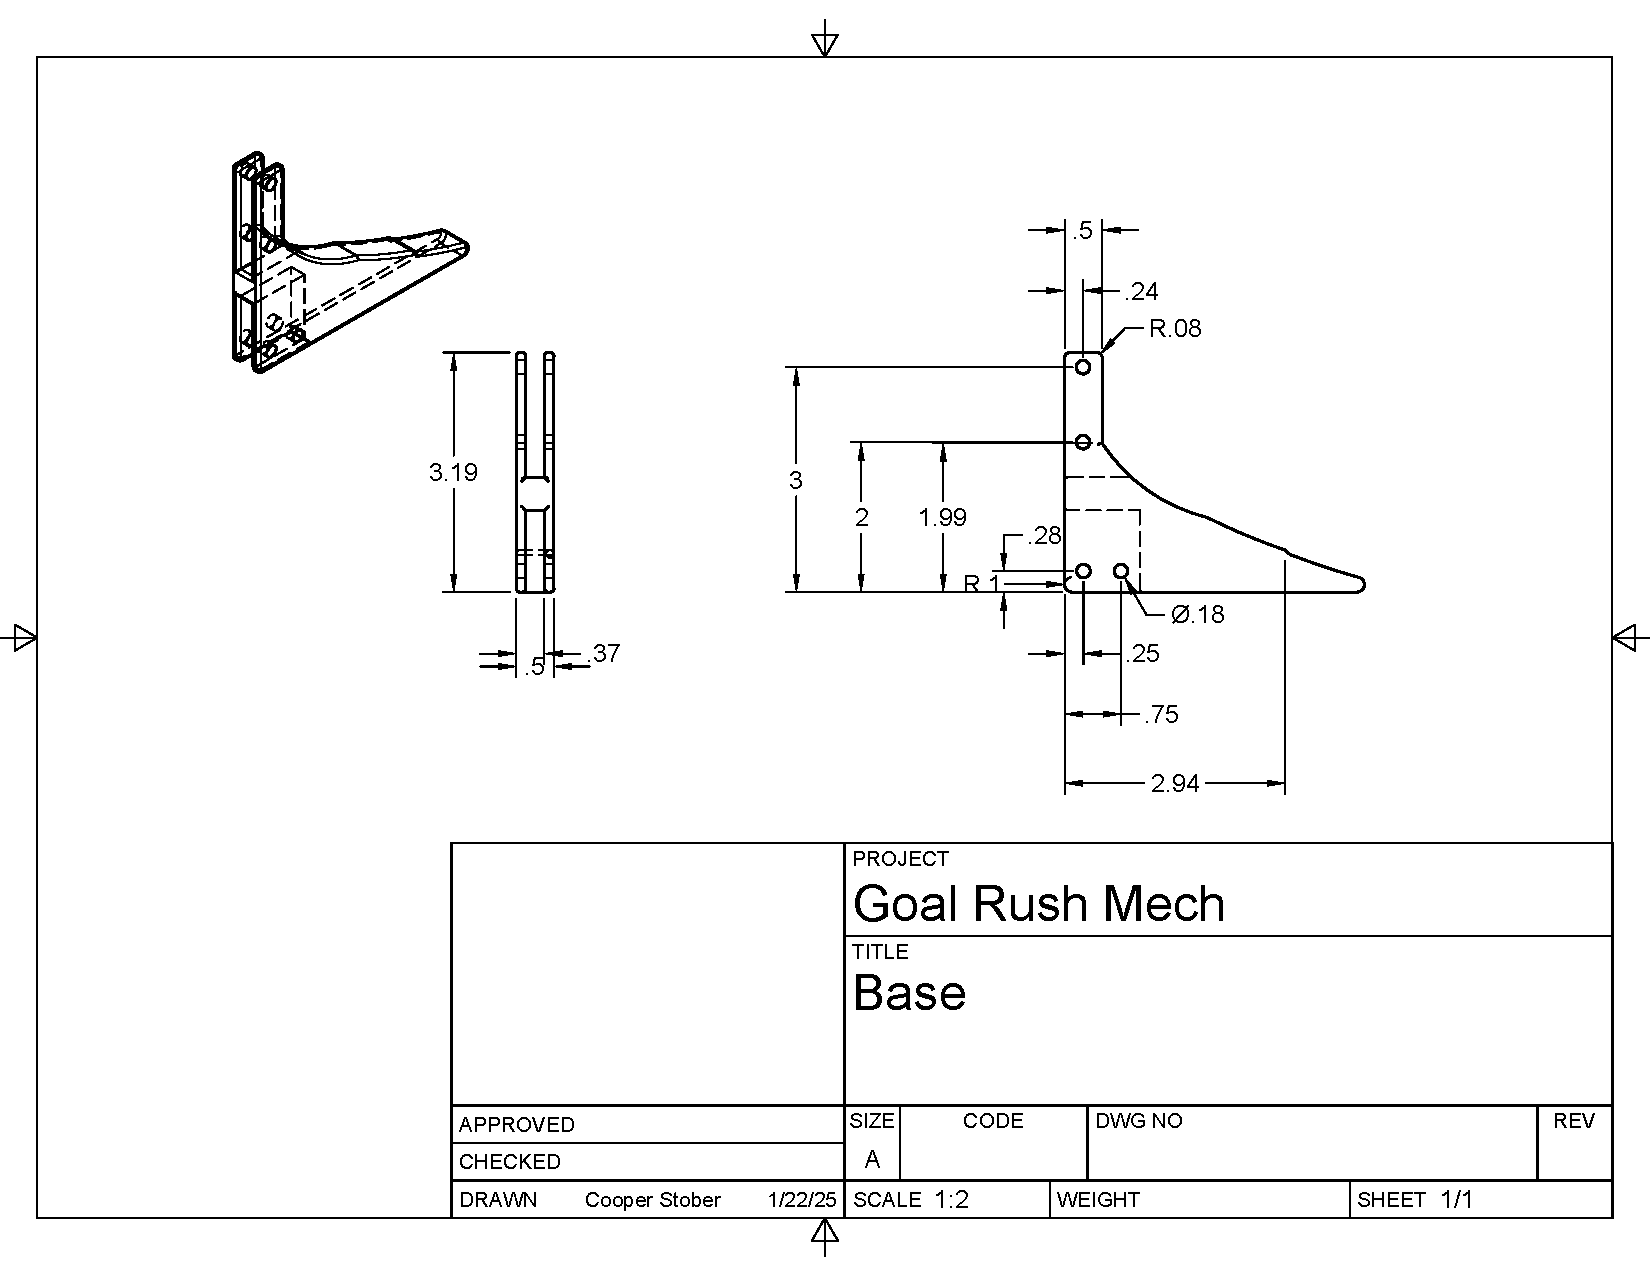
\includegraphics[width=\textheight, angle =90 ]{images/Subassemblies Drawings and Parts/Base Drawing.pdf}
    \caption{Enter Caption}
    \label{fig:enter-label}
\end{figure}

\begin{figure}
    \centering
    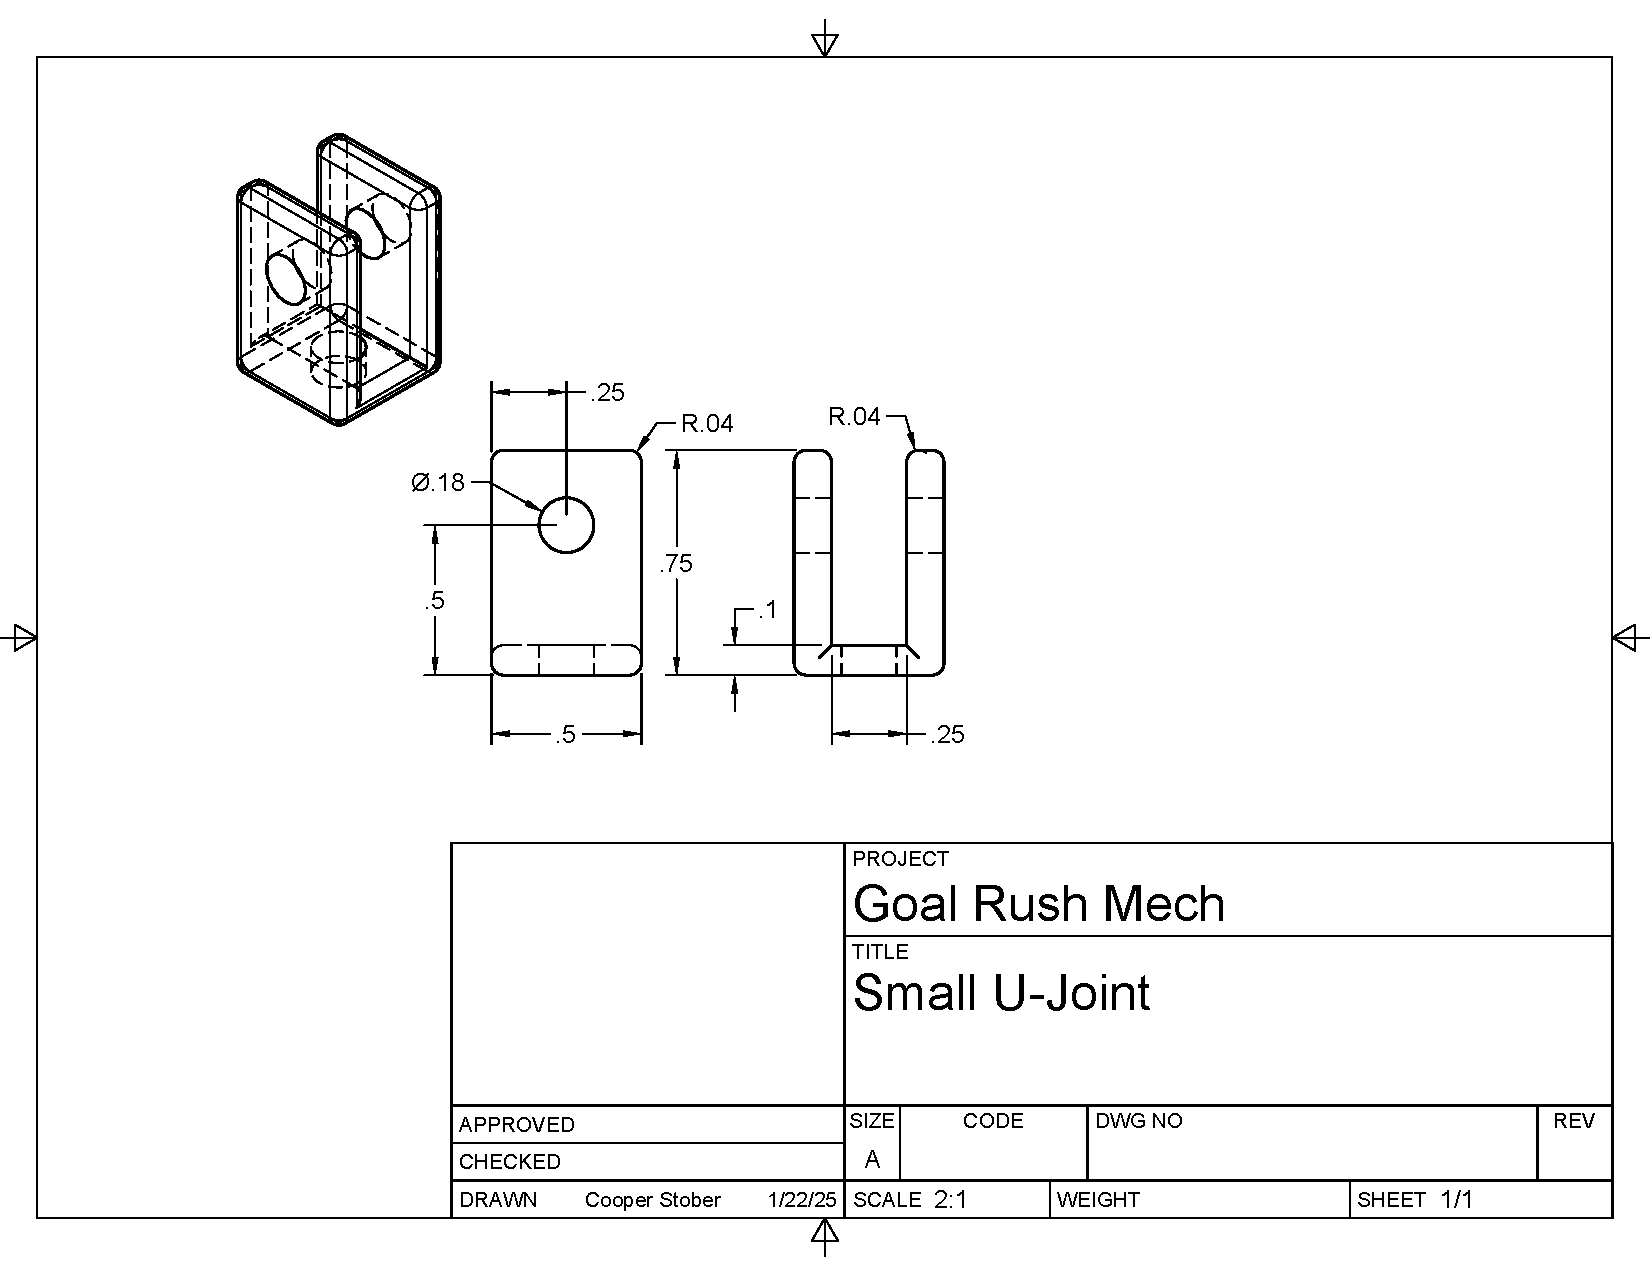
\includegraphics[width=\textheight, angle = 90]{images/Subassemblies Drawings and Parts/Small U-Joint Drawing.pdf}
    \caption{Enter Caption}
    \label{fig:enter-label}
\end{figure}

\begin{figure}
    \centering
    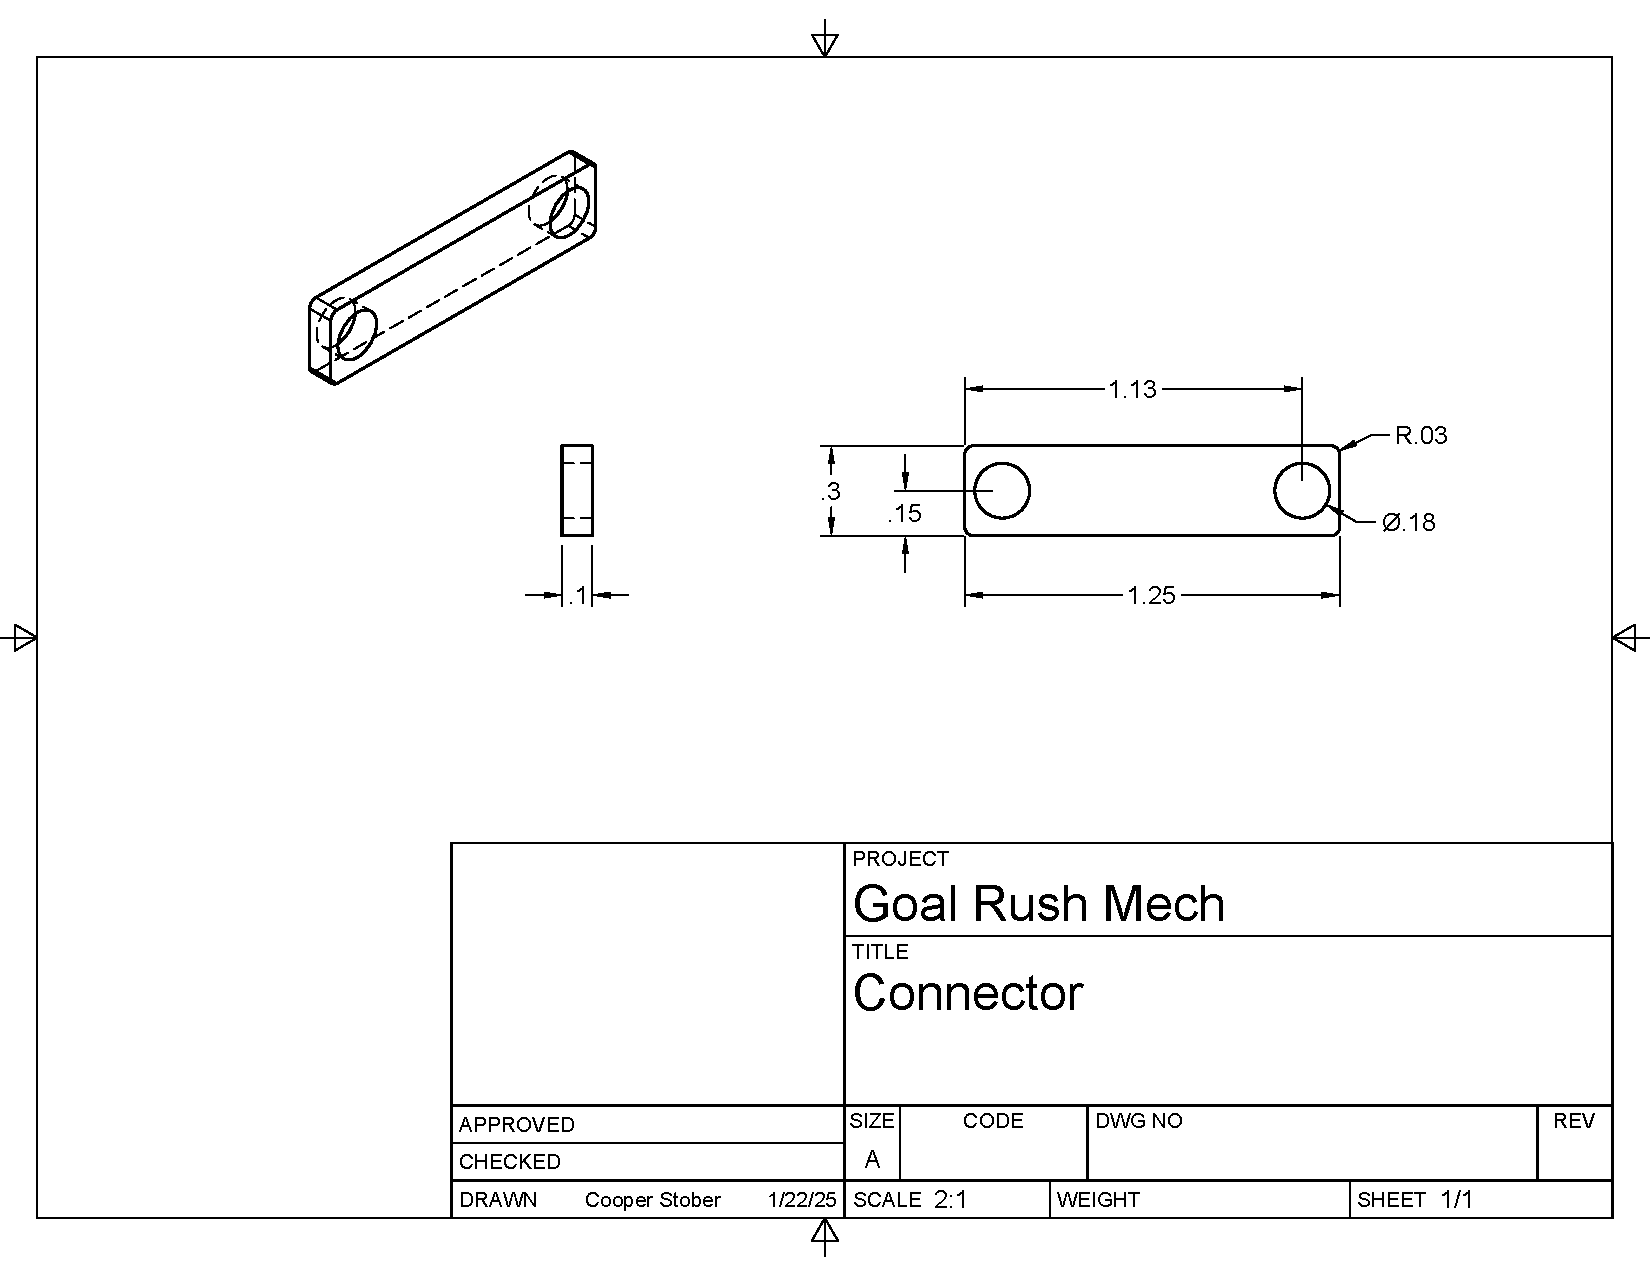
\includegraphics[width=\textheight, angle =90 ]{images/Subassemblies Drawings and Parts/Connector Drawing.pdf}
    \caption{Enter Caption}
    \label{fig:enter-label}
\end{figure}

\begin{figure}
    \centering
    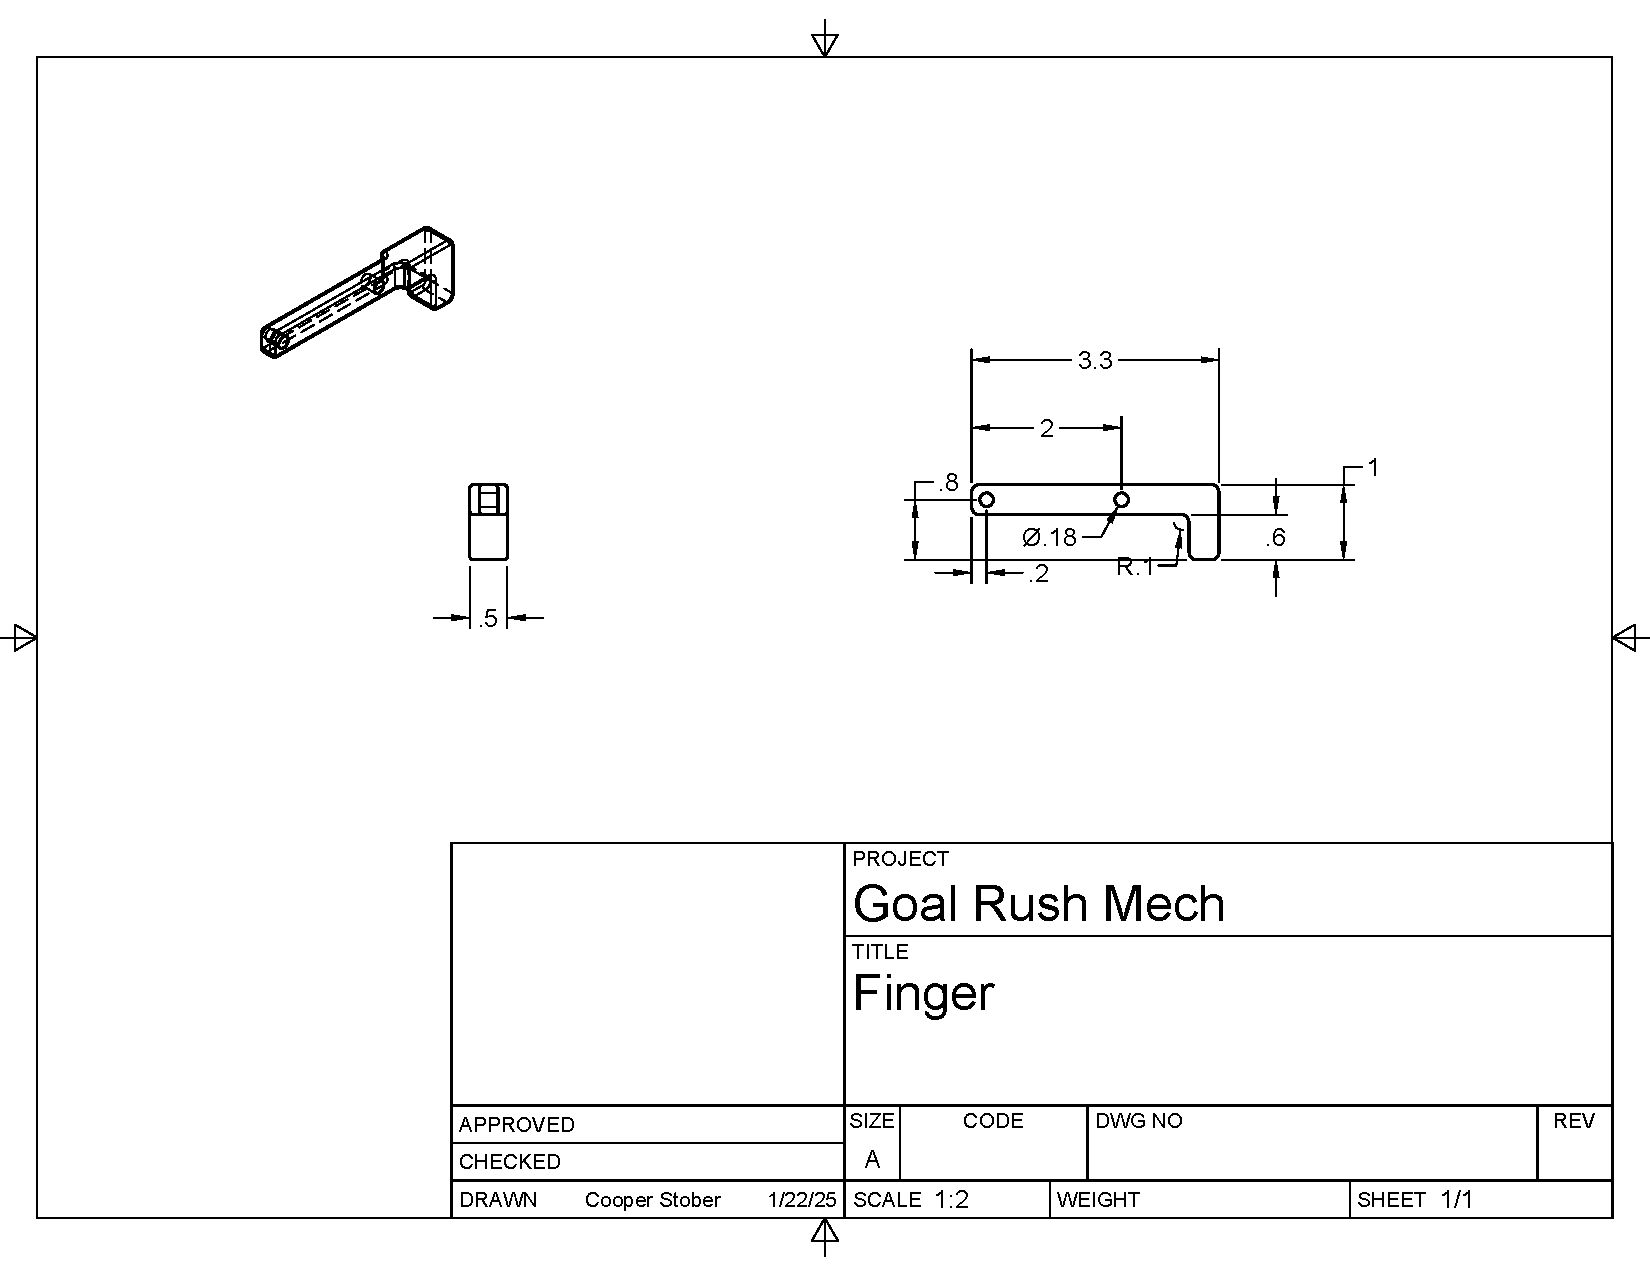
\includegraphics[width=\textheight, angle =90 ]{images/Subassemblies Drawings and Parts/Finger Drawing.pdf}
    \caption{Enter Caption}
    \label{fig:enter-label}
\end{figure}

\begin{figure}
    \centering
    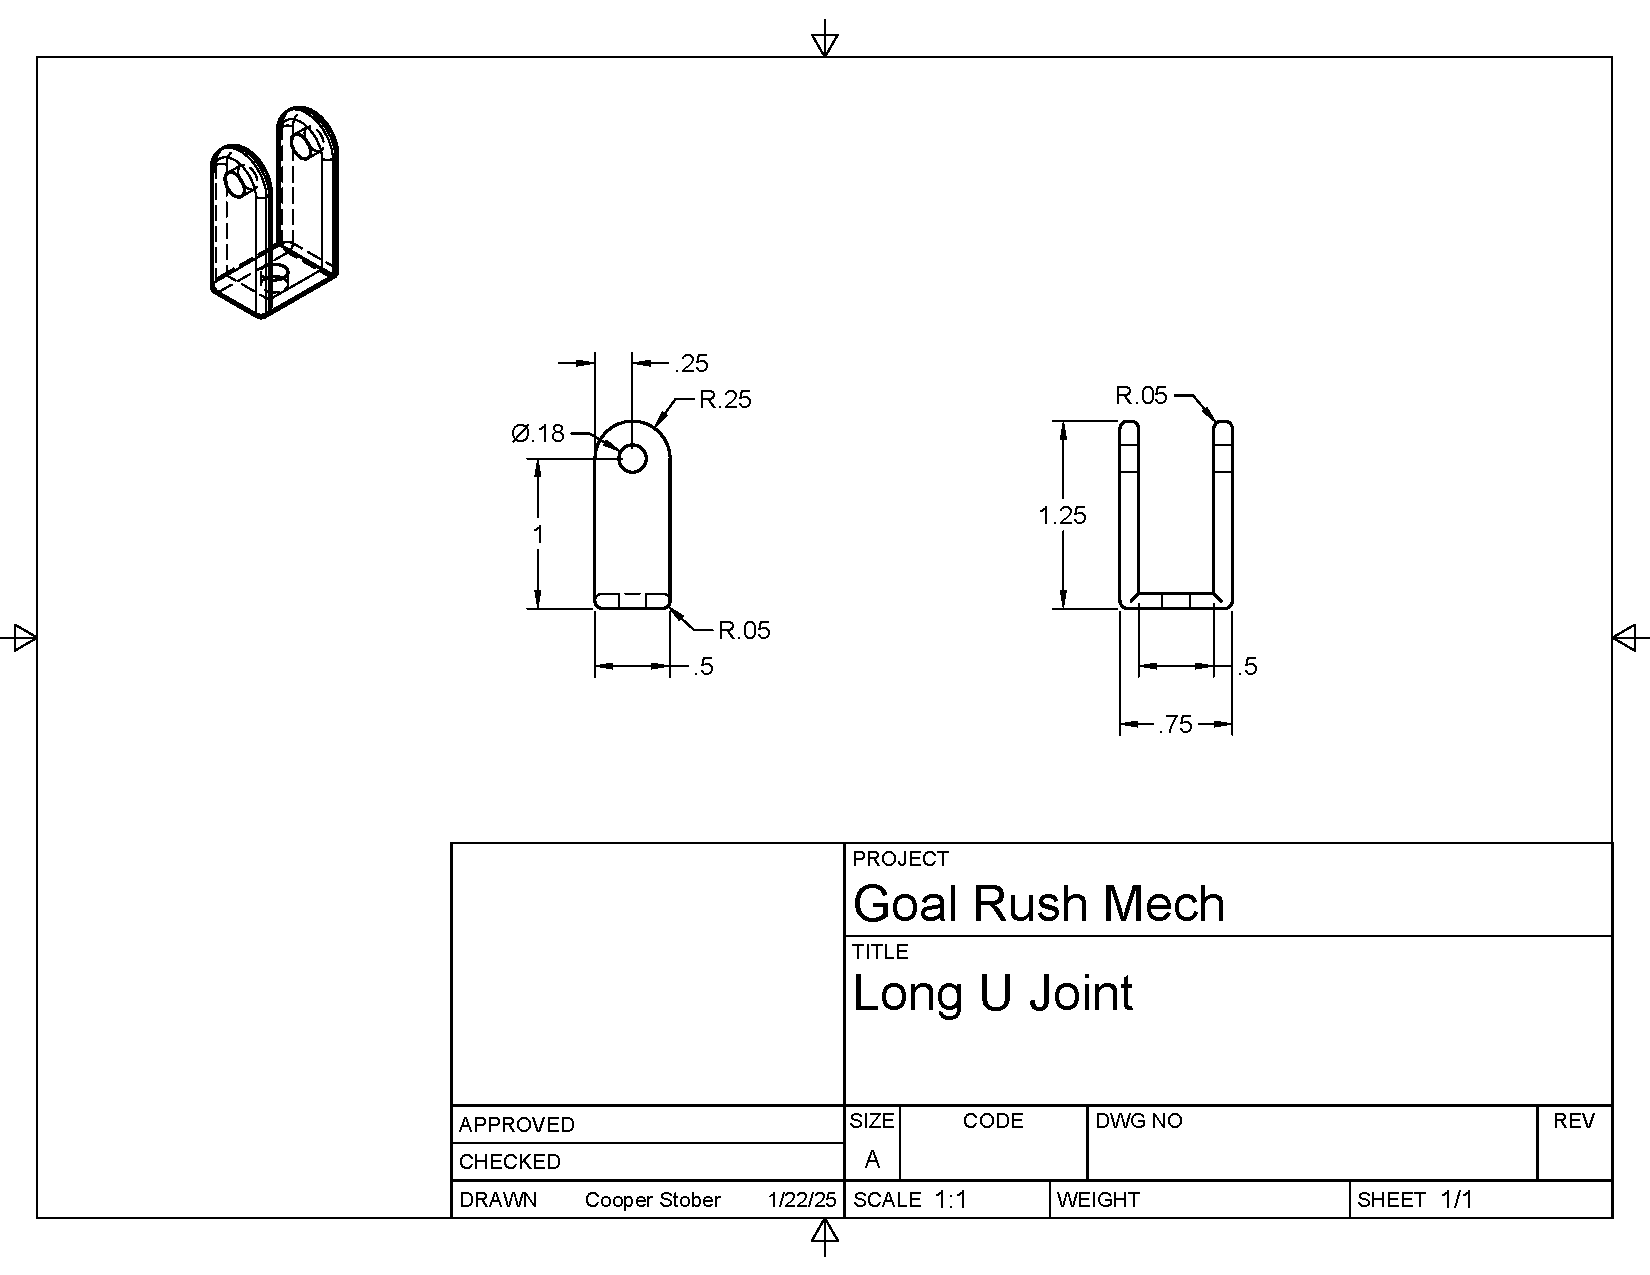
\includegraphics[width=\textheight, angle=90]{images/Subassemblies Drawings and Parts/Long U Joint Drawing.pdf}
    \caption{Enter Caption}
    \label{fig:enter-label}
\end{figure}

\begin{figure}
    \centering
    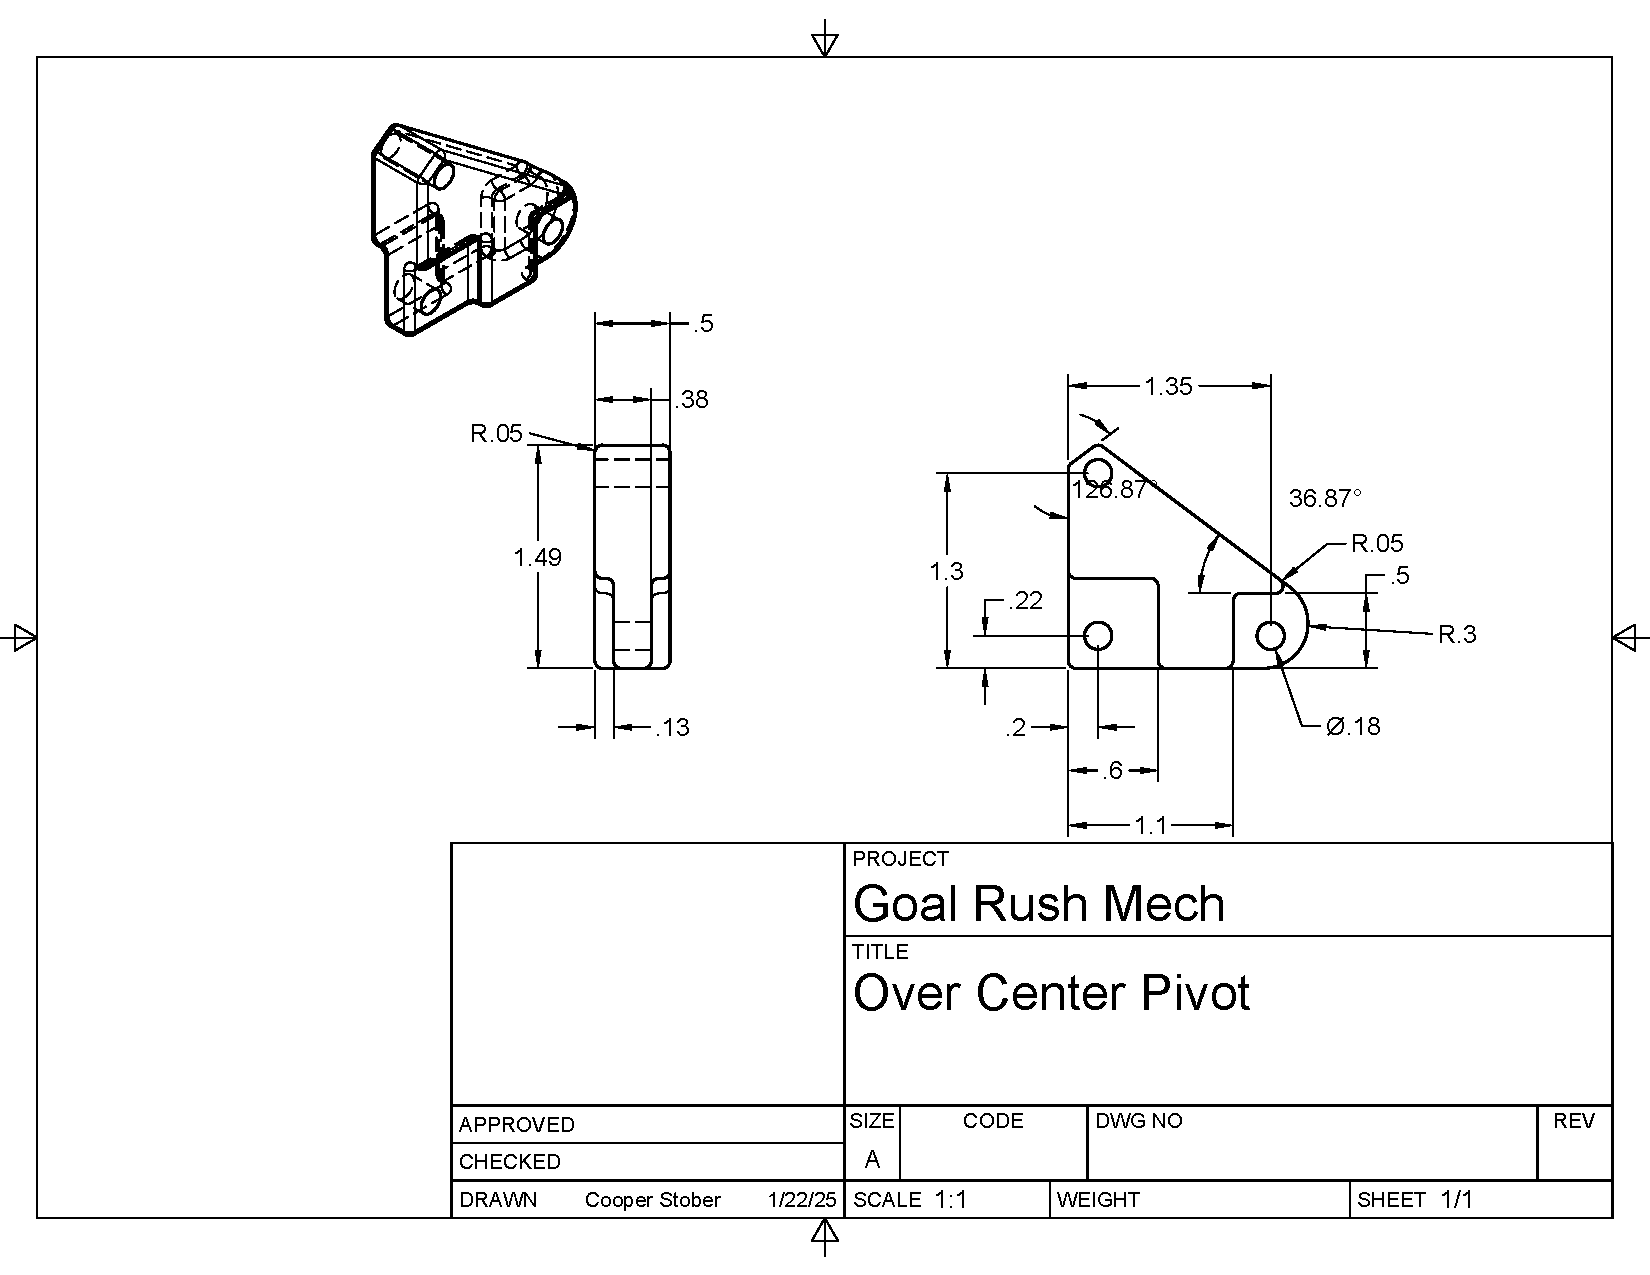
\includegraphics[width=\textheight, angle =90]{images/Subassemblies Drawings and Parts/Over Center Pivot Drawing.pdf}
    \caption{Enter Caption}
    \label{fig:enter-label}
\end{figure}


\begin{figure}
    \centering
    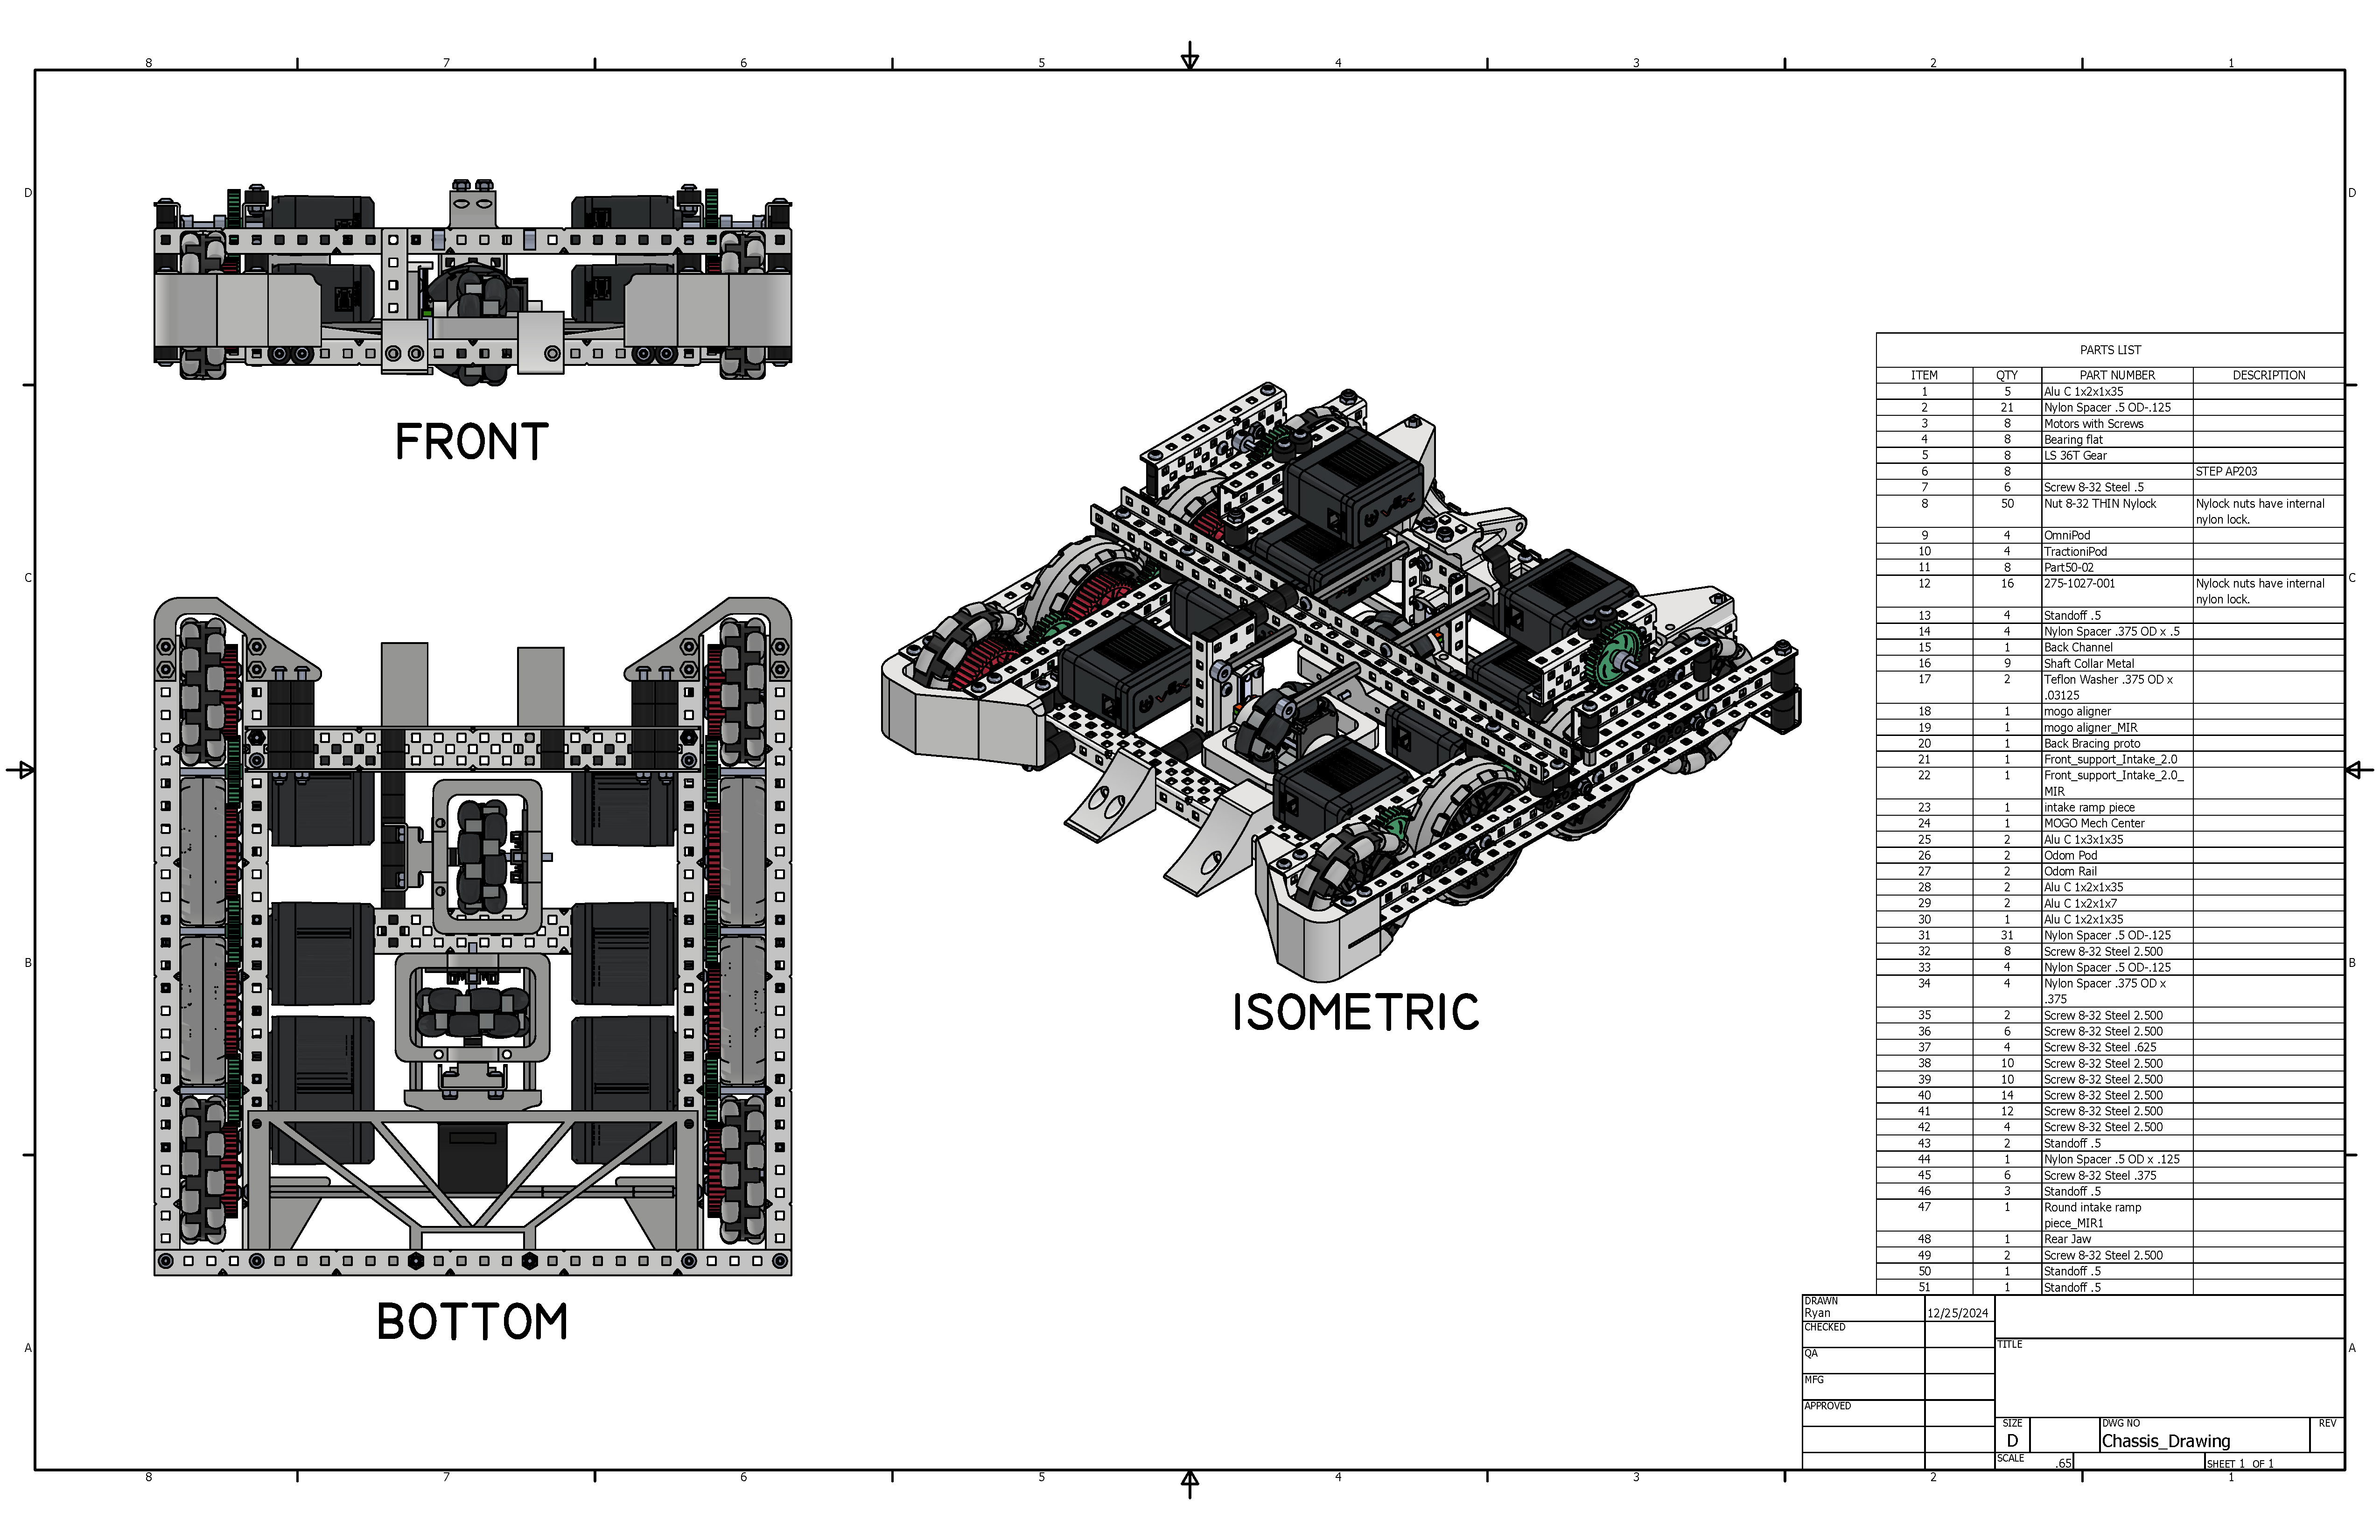
\includegraphics[width=\textheight, angle =90 ]{images/Subassemblies Drawings and Parts/Chassis_Drawing.pdf}
    \caption{Enter Caption}
    \label{fig:enter-label}
\end{figure}



\begin{figure}
    \centering
    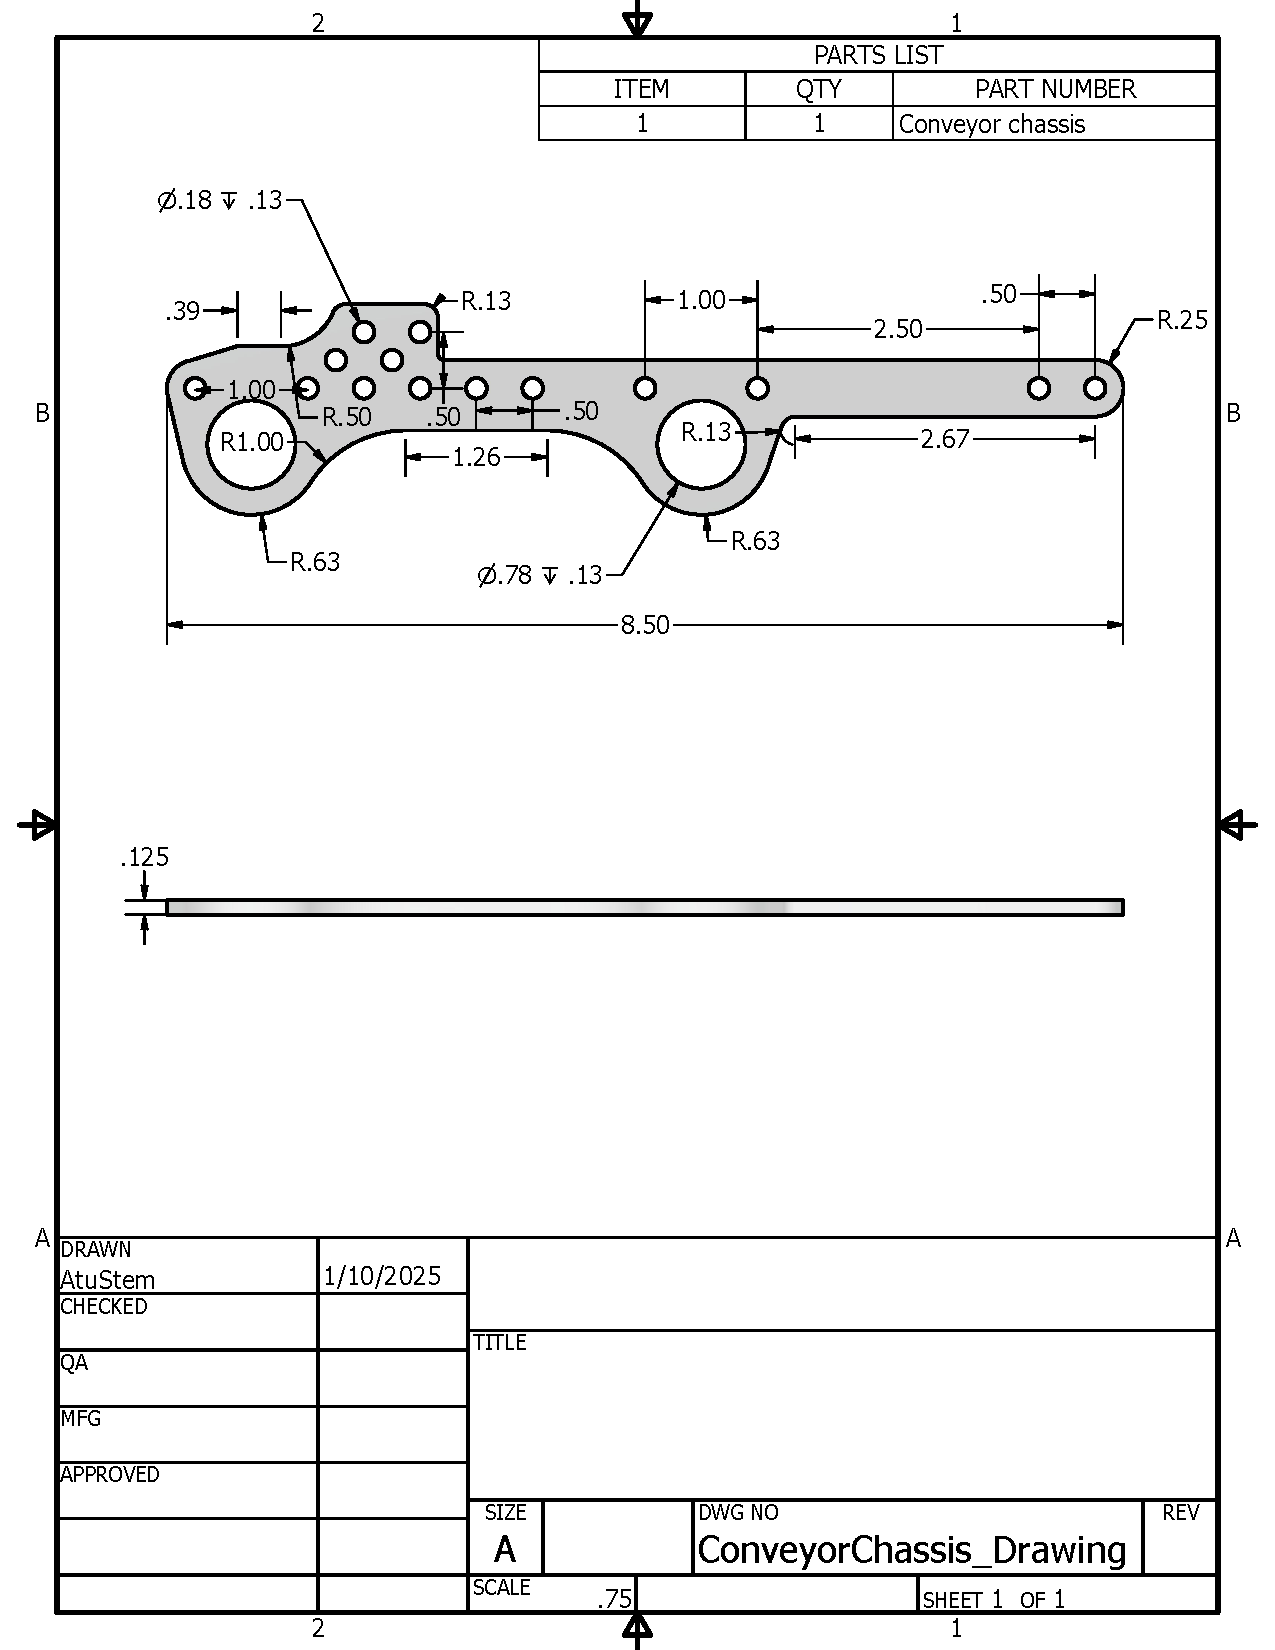
\includegraphics[width=\textwidth]{images/Subassemblies Drawings and Parts/ConveyorChassis_Drawing.pdf}
    \caption{Enter Caption}
    \label{fig:enter-label}
\end{figure}



\begin{figure}
    \centering
    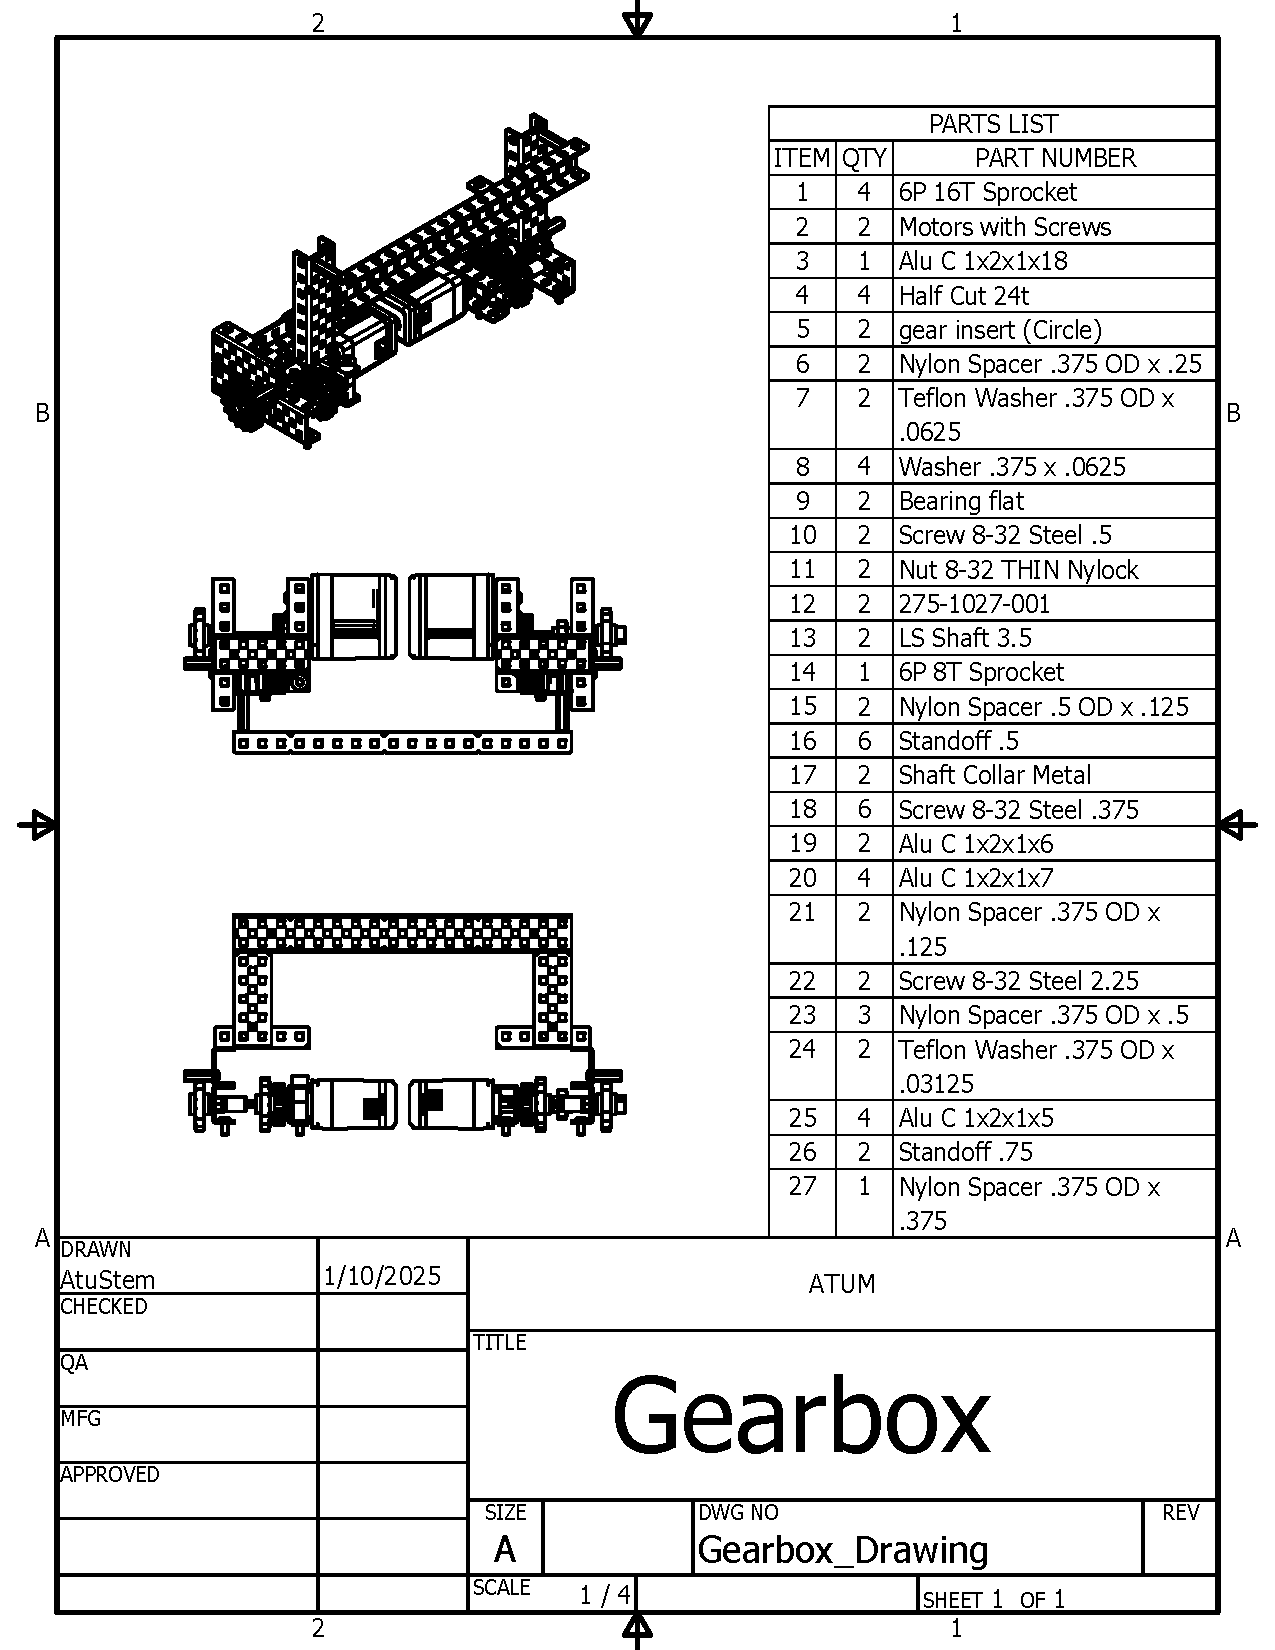
\includegraphics[width=1\linewidth]{images/Subassemblies Drawings and Parts/Gearbox_Drawing.pdf}
    \caption{Enter Caption}
    \label{fig:enter-label}
\end{figure}

\begin{figure}
    \centering
    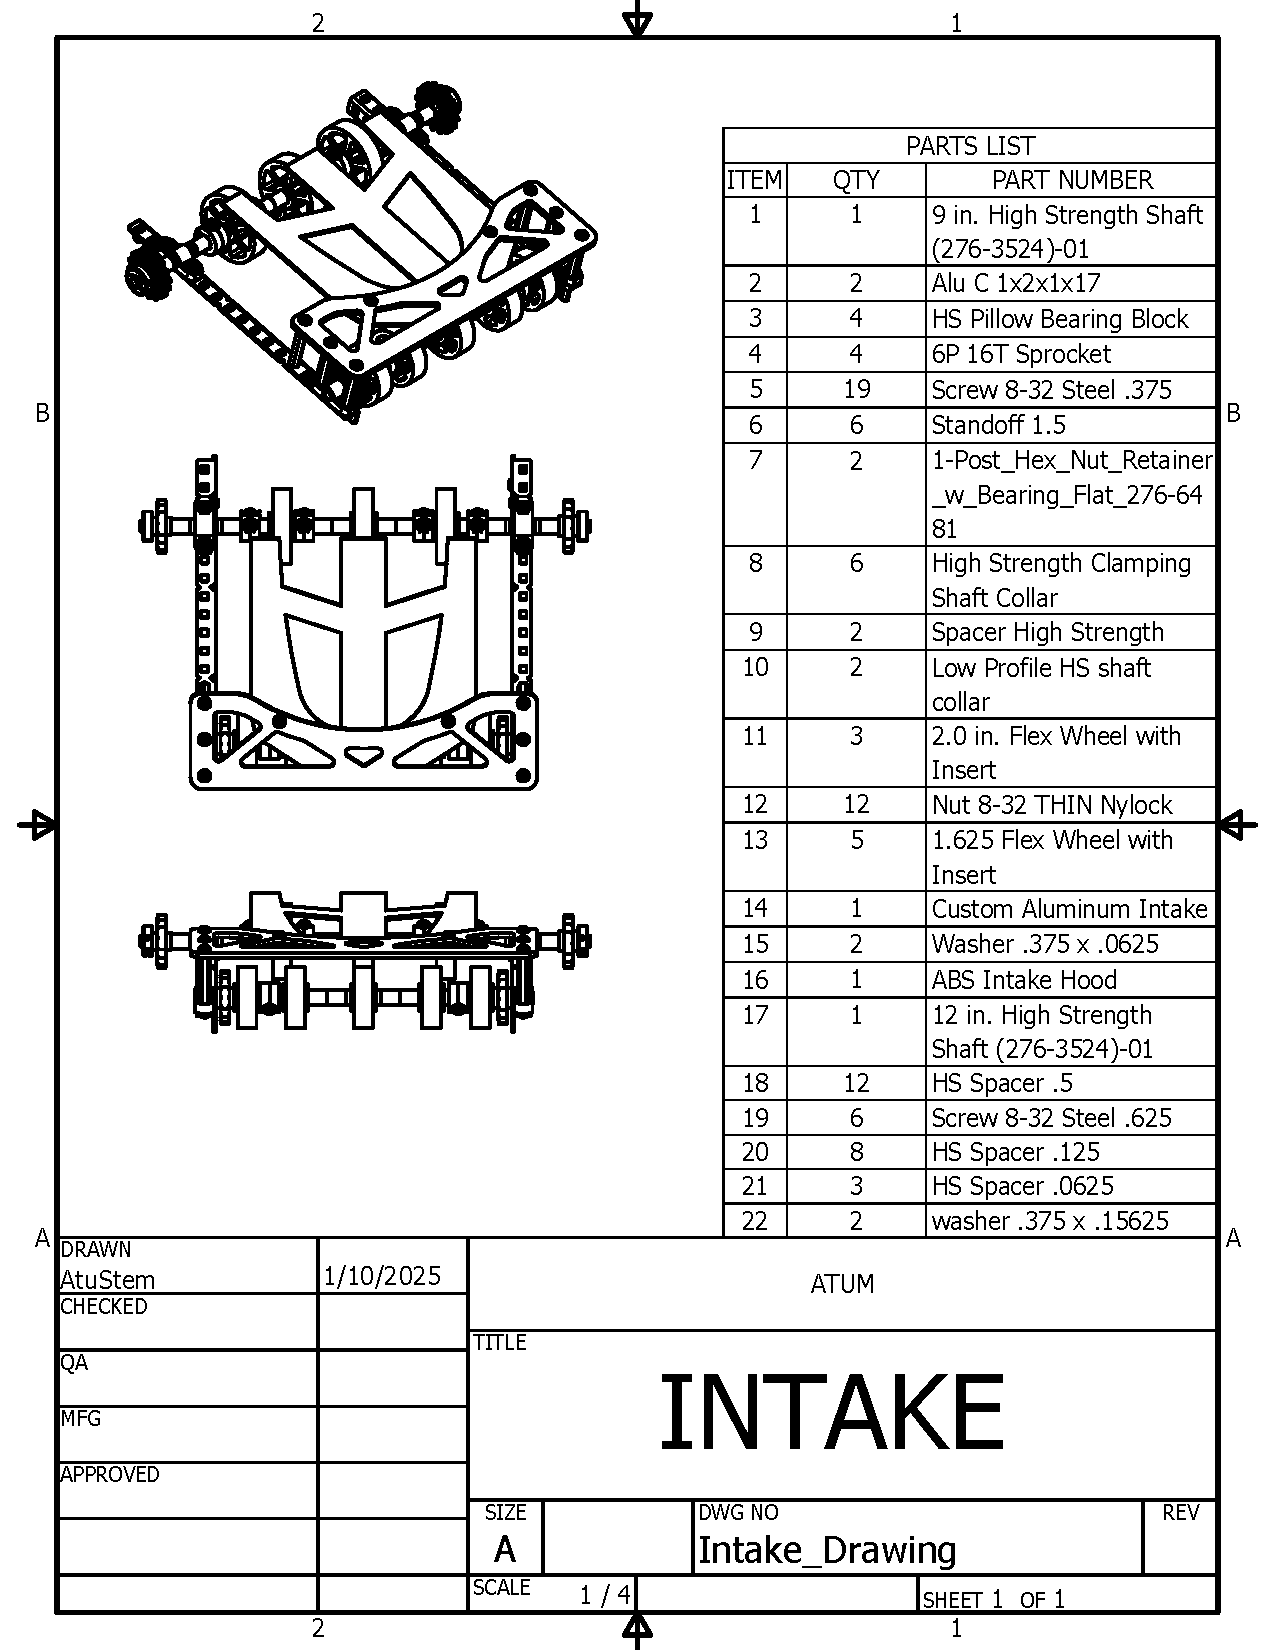
\includegraphics[width=1\linewidth]{images/Subassemblies Drawings and Parts/Intake_Drawing.pdf}
    \caption{Enter Caption}
    \label{fig:enter-label}
\end{figure}

\begin{figure}
    \centering
    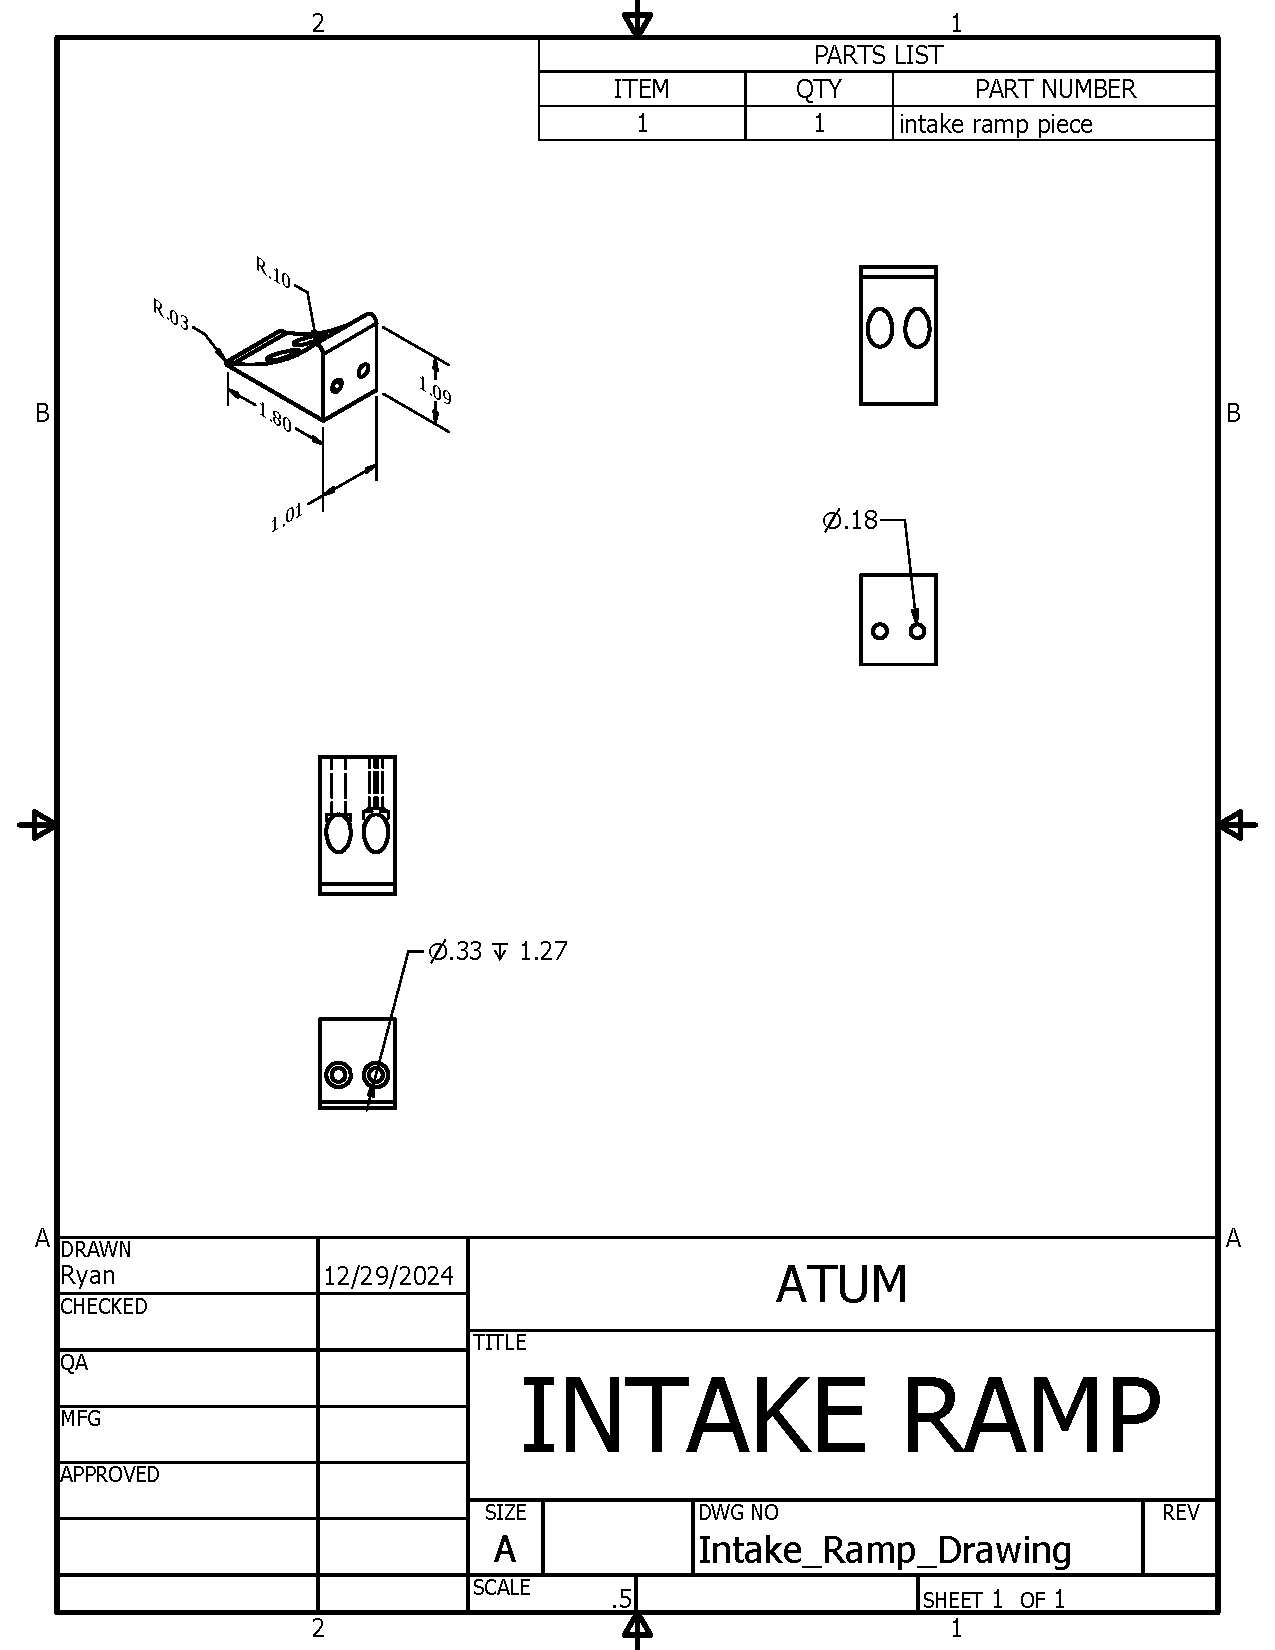
\includegraphics[width=1\linewidth]{images/Subassemblies Drawings and Parts/Intake_Ramp_Drawing.pdf}
    \caption{Enter Caption}
    \label{fig:enter-label}
\end{figure}

\begin{figure}
    \centering
    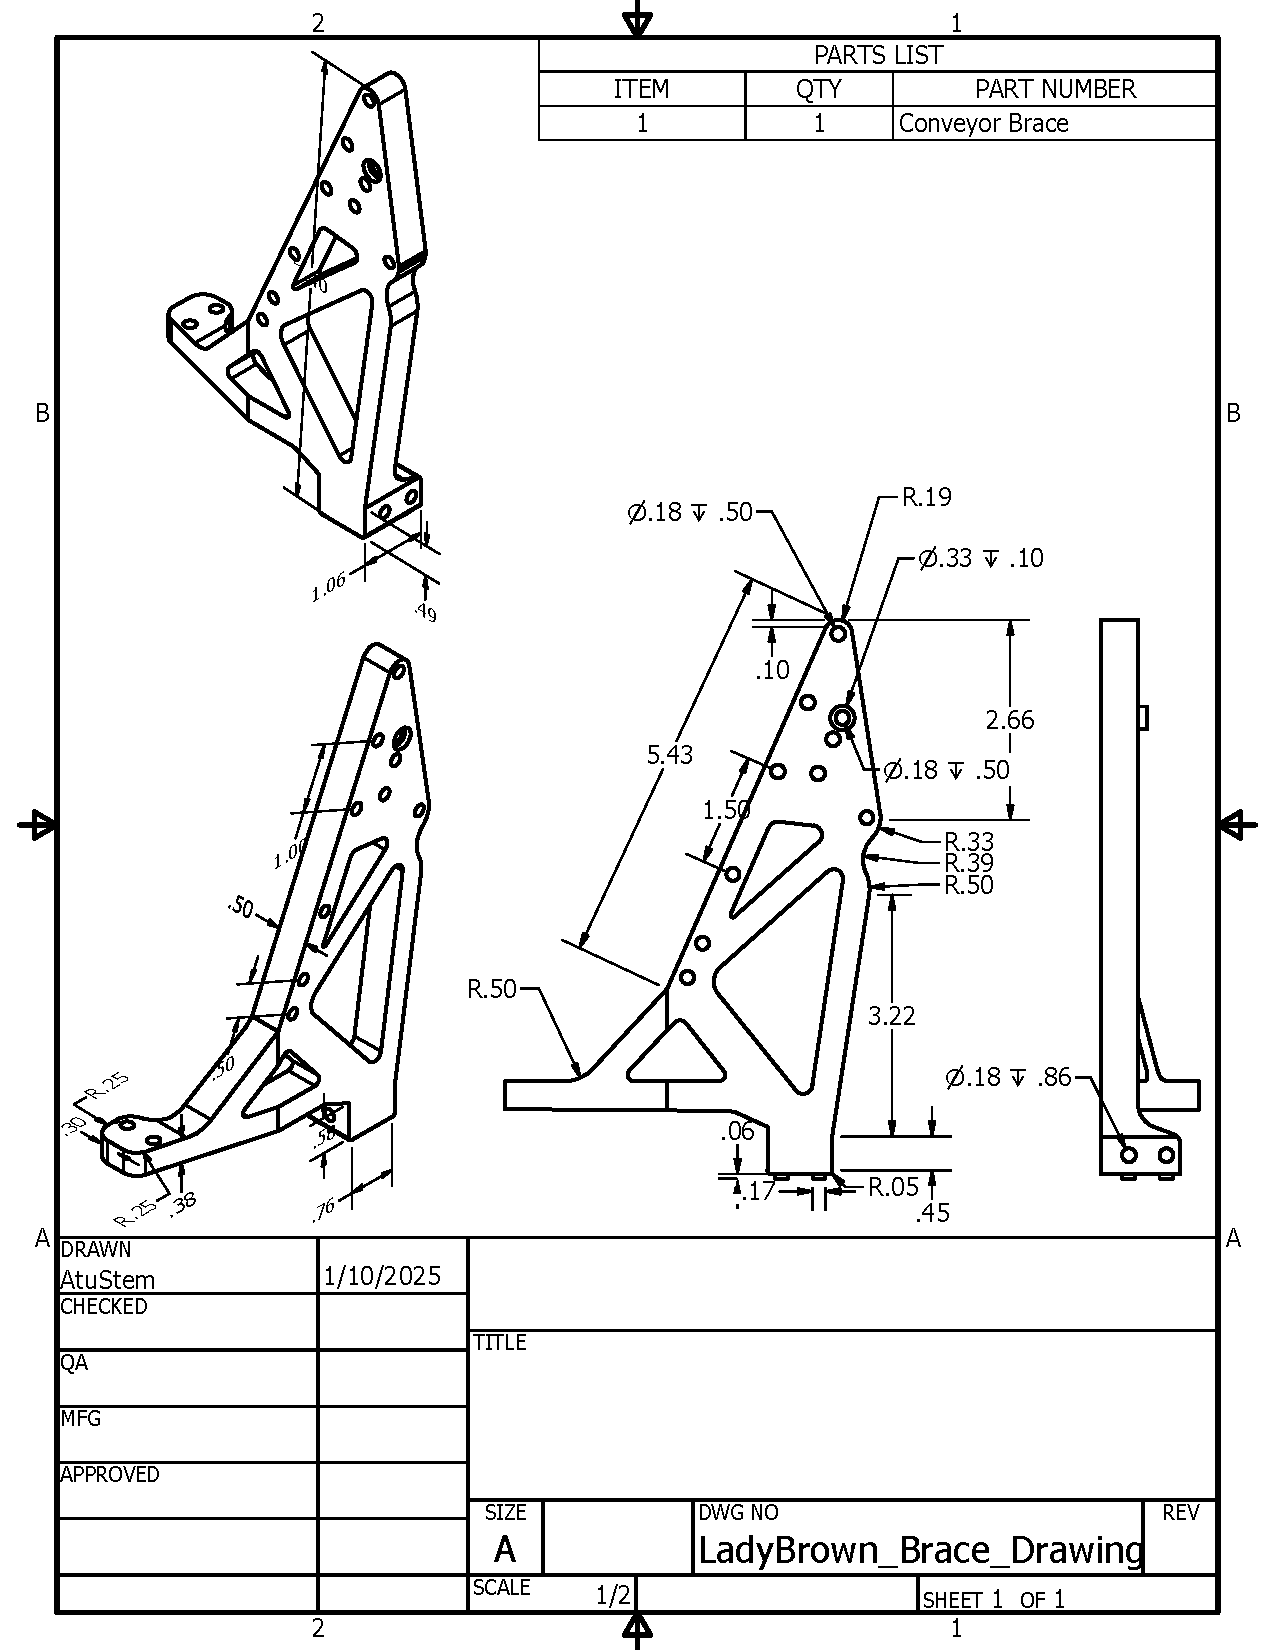
\includegraphics[width=1\linewidth]{images/Subassemblies Drawings and Parts/LadyBrown_Brace_Drawing.pdf}
    \caption{Enter Caption}
    \label{fig:enter-label}
\end{figure}

\begin{figure}
    \centering
    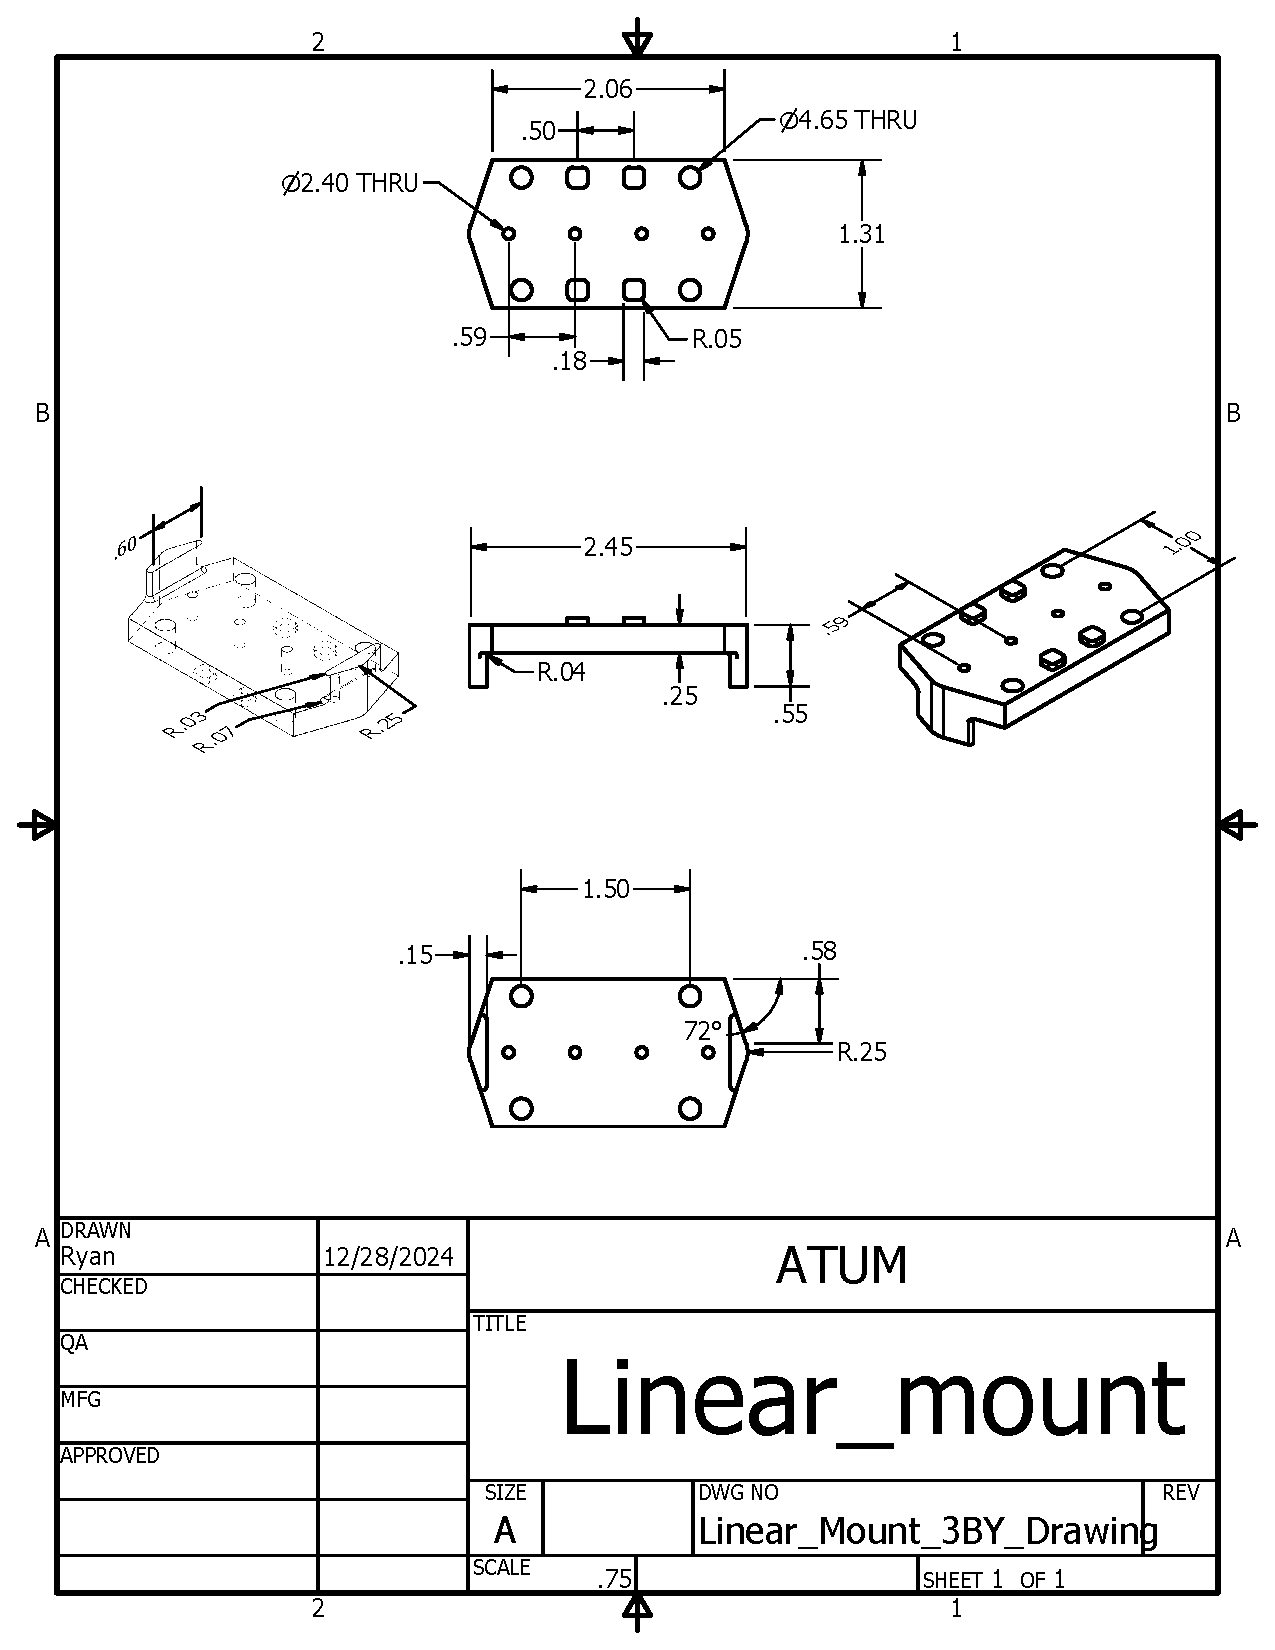
\includegraphics[width=1\linewidth]{images/Subassemblies Drawings and Parts/Linear_Mount_3BY_Drawing.pdf}
    \caption{Enter Caption}
    \label{fig:enter-label}
\end{figure}

\begin{figure}
    \centering
    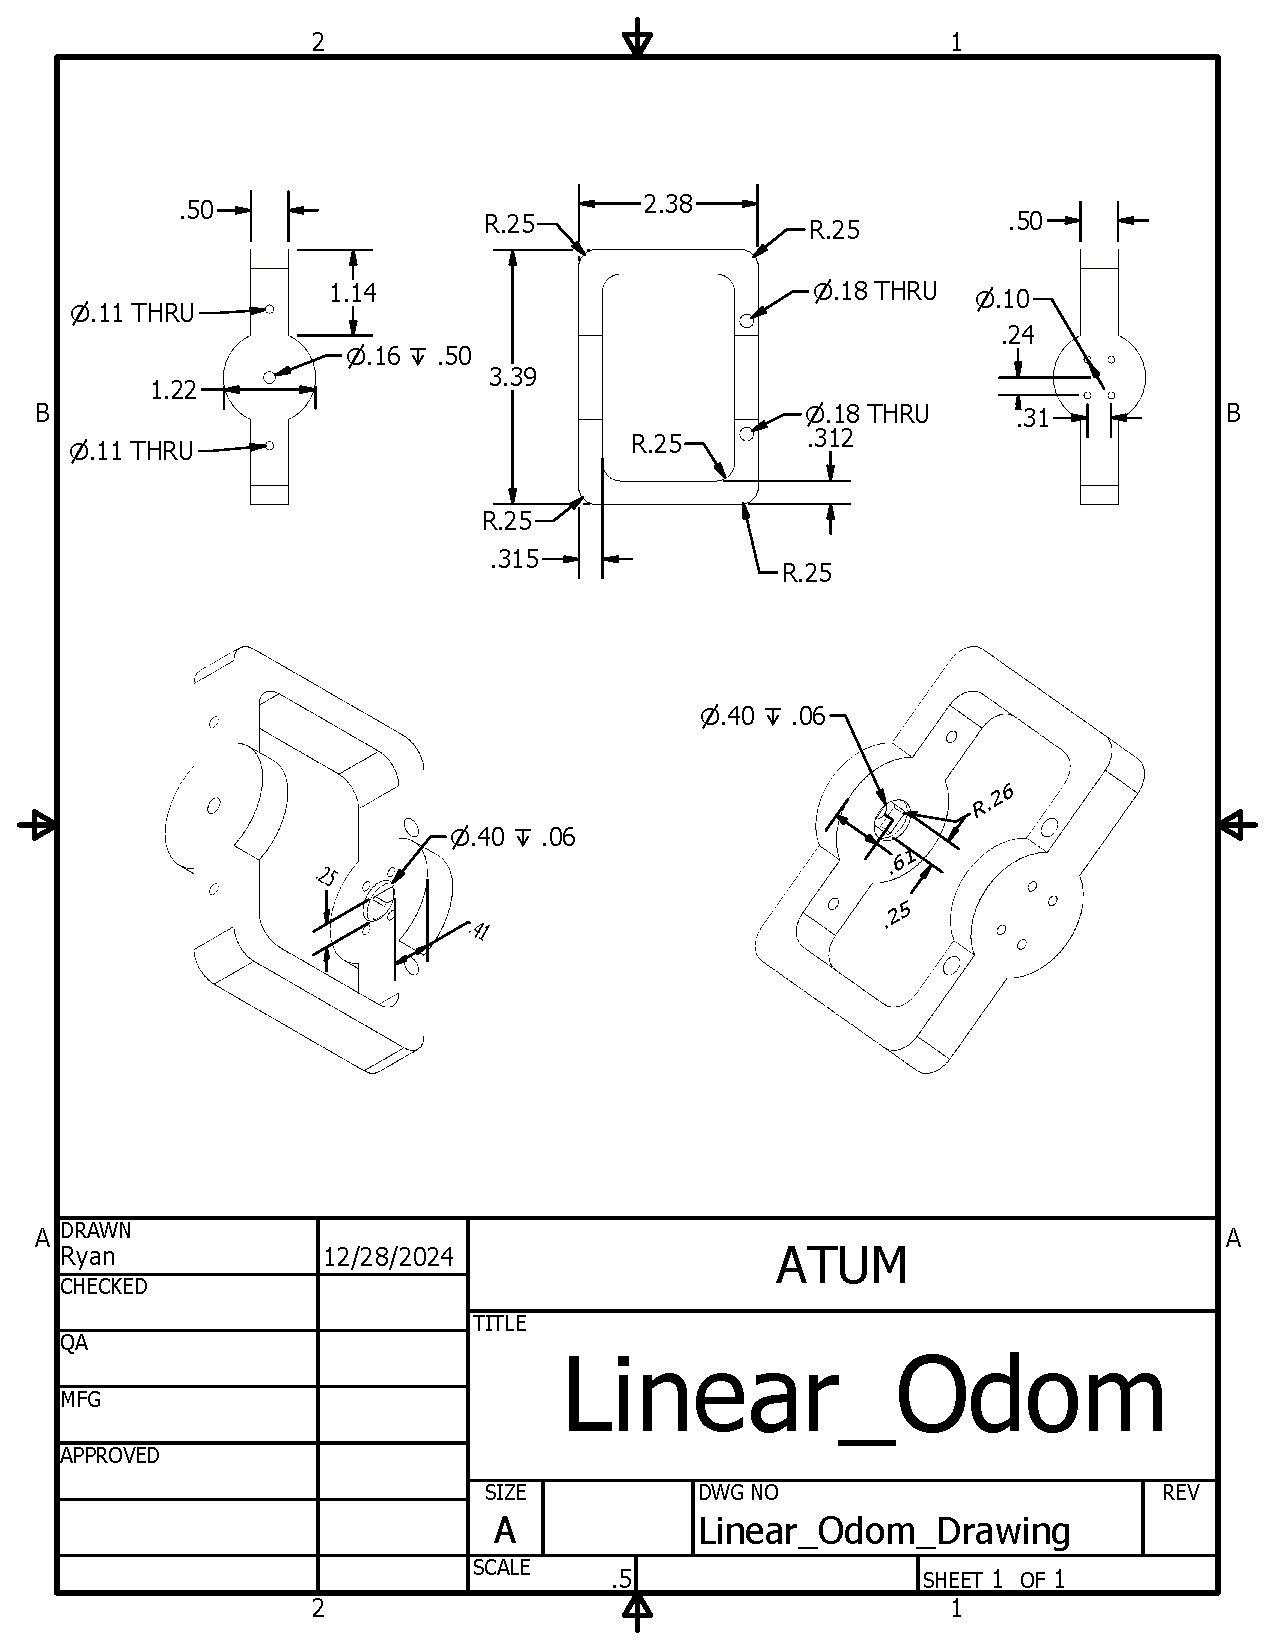
\includegraphics[width=1\linewidth]{images/Subassemblies Drawings and Parts/Linear_Odom_Drawing.pdf}
    \caption{Enter Caption}
    \label{fig:enter-label}
\end{figure}



\begin{figure}
    \centering
    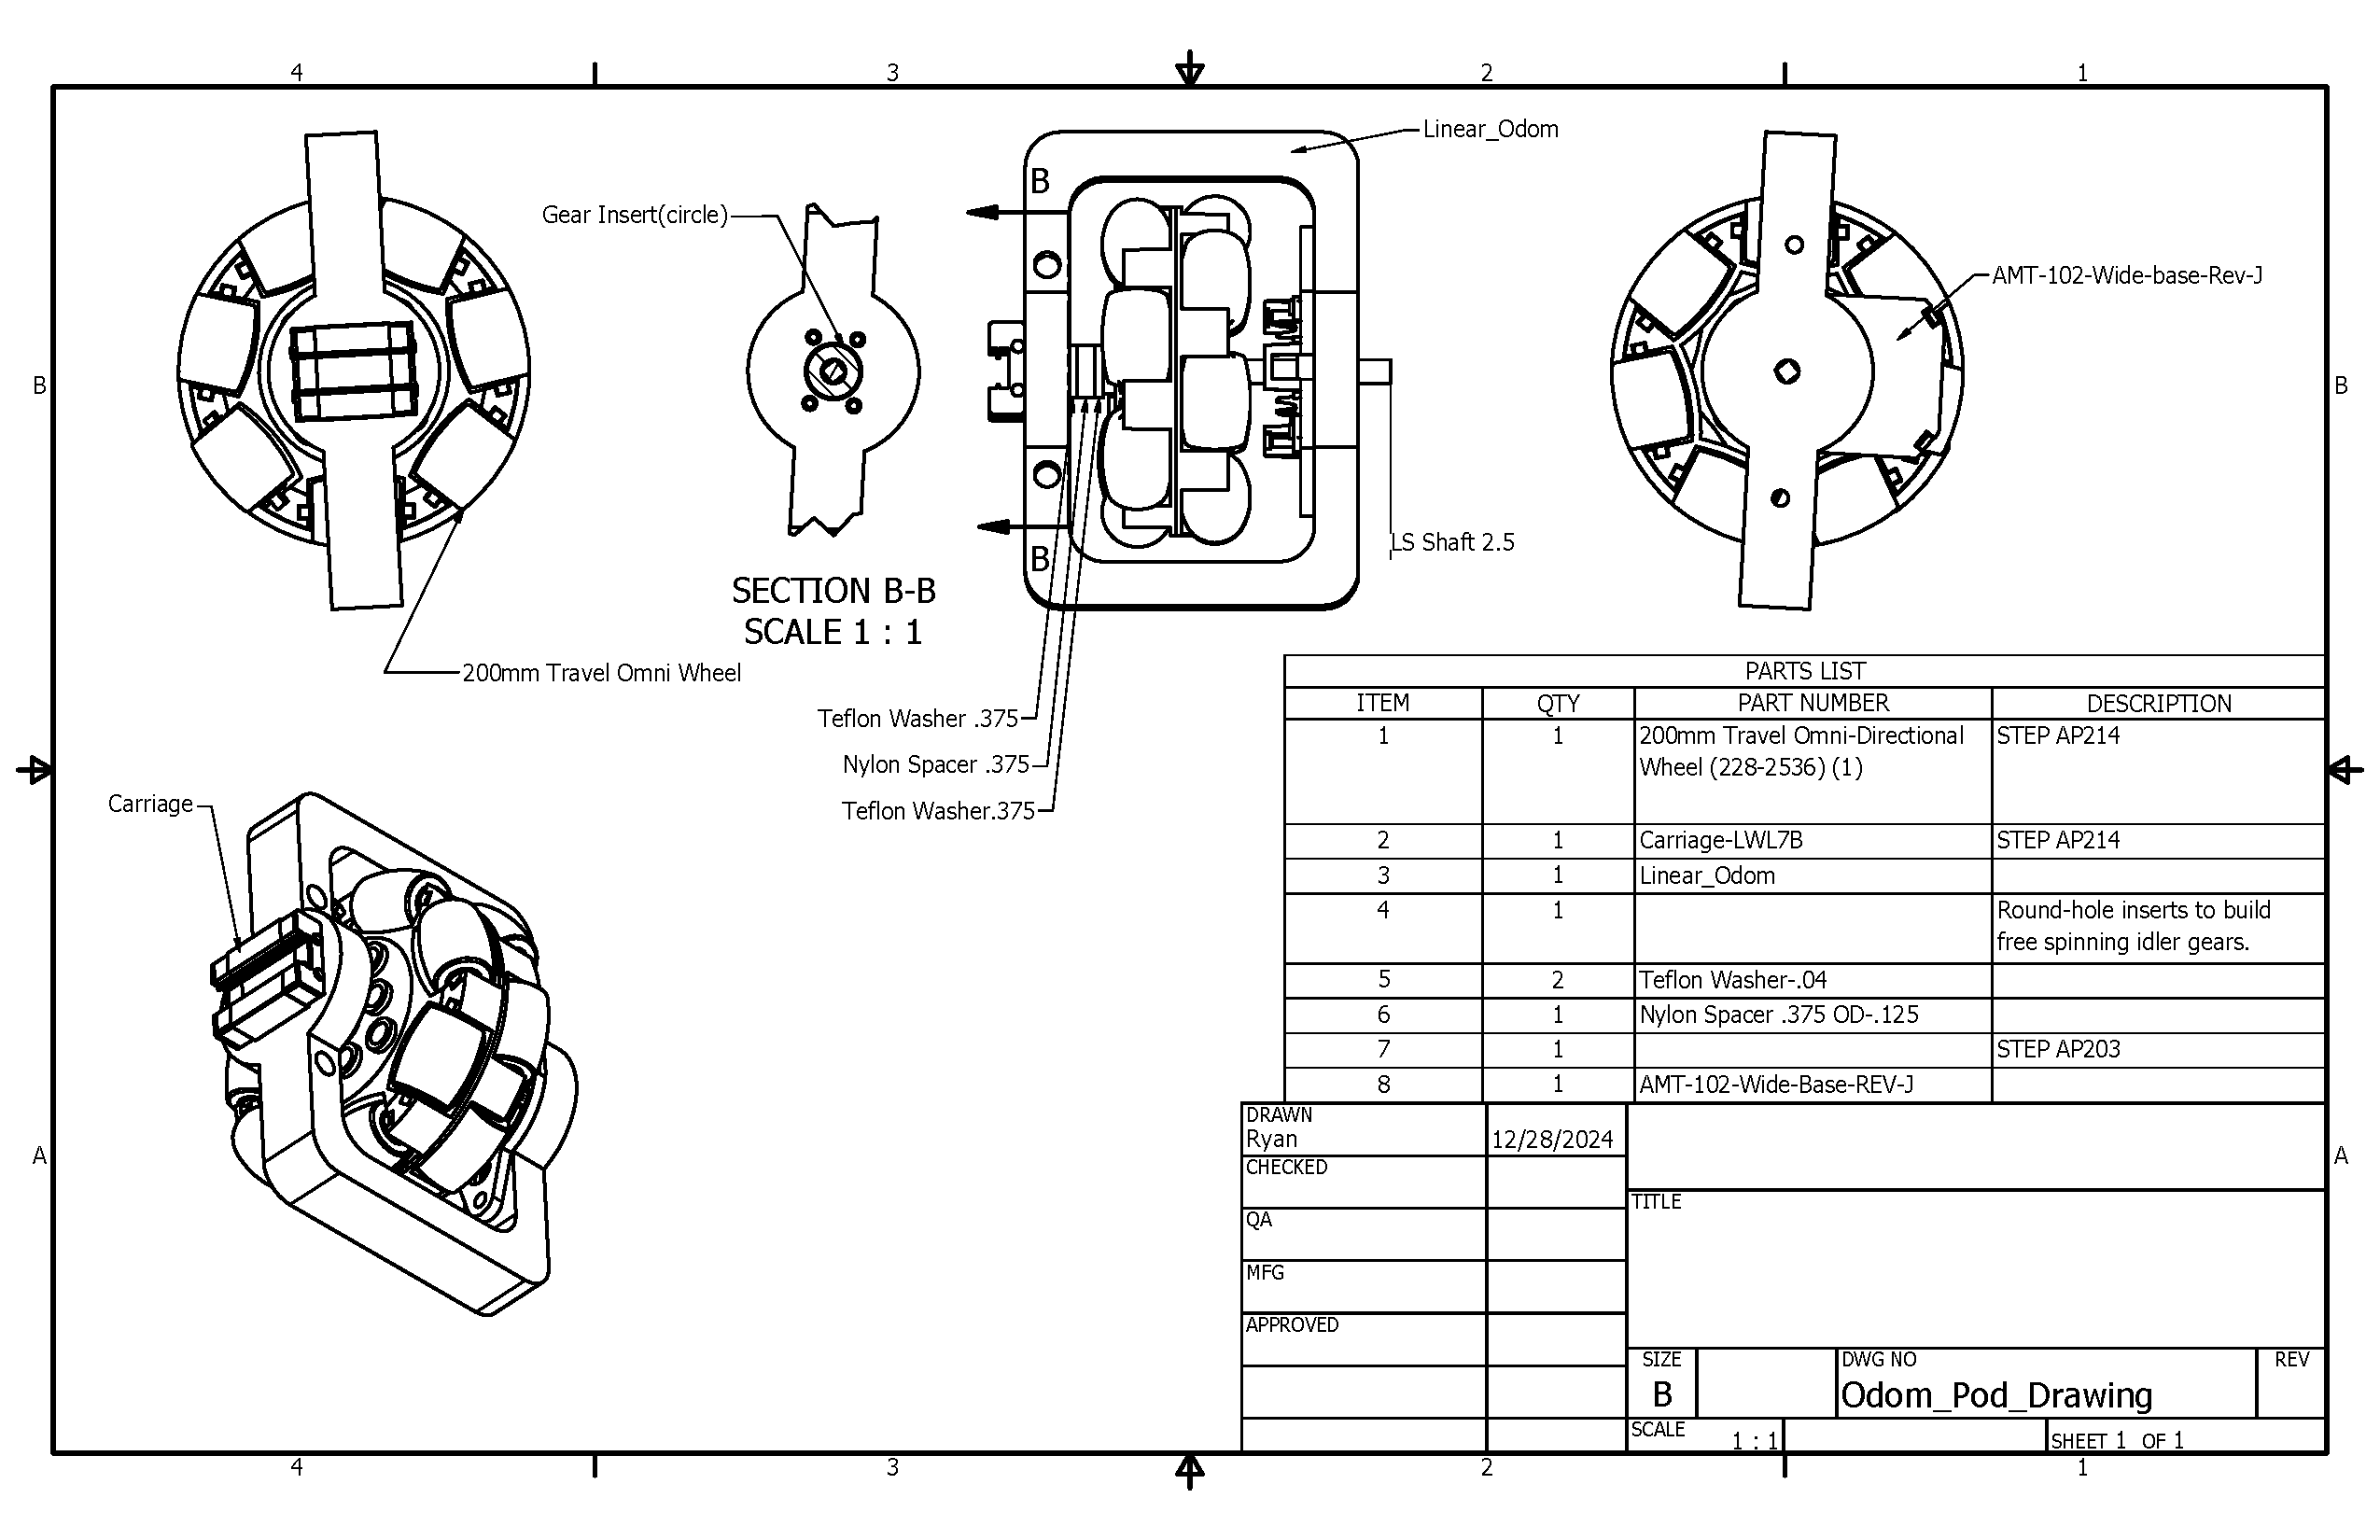
\includegraphics[width=\textheight, angle=90]{images/Subassemblies Drawings and Parts/Odom_Pod_Drawing.pdf}
    \caption{Enter Caption}
    \label{fig:enter-label}
\end{figure}

\begin{figure}
    \centering
    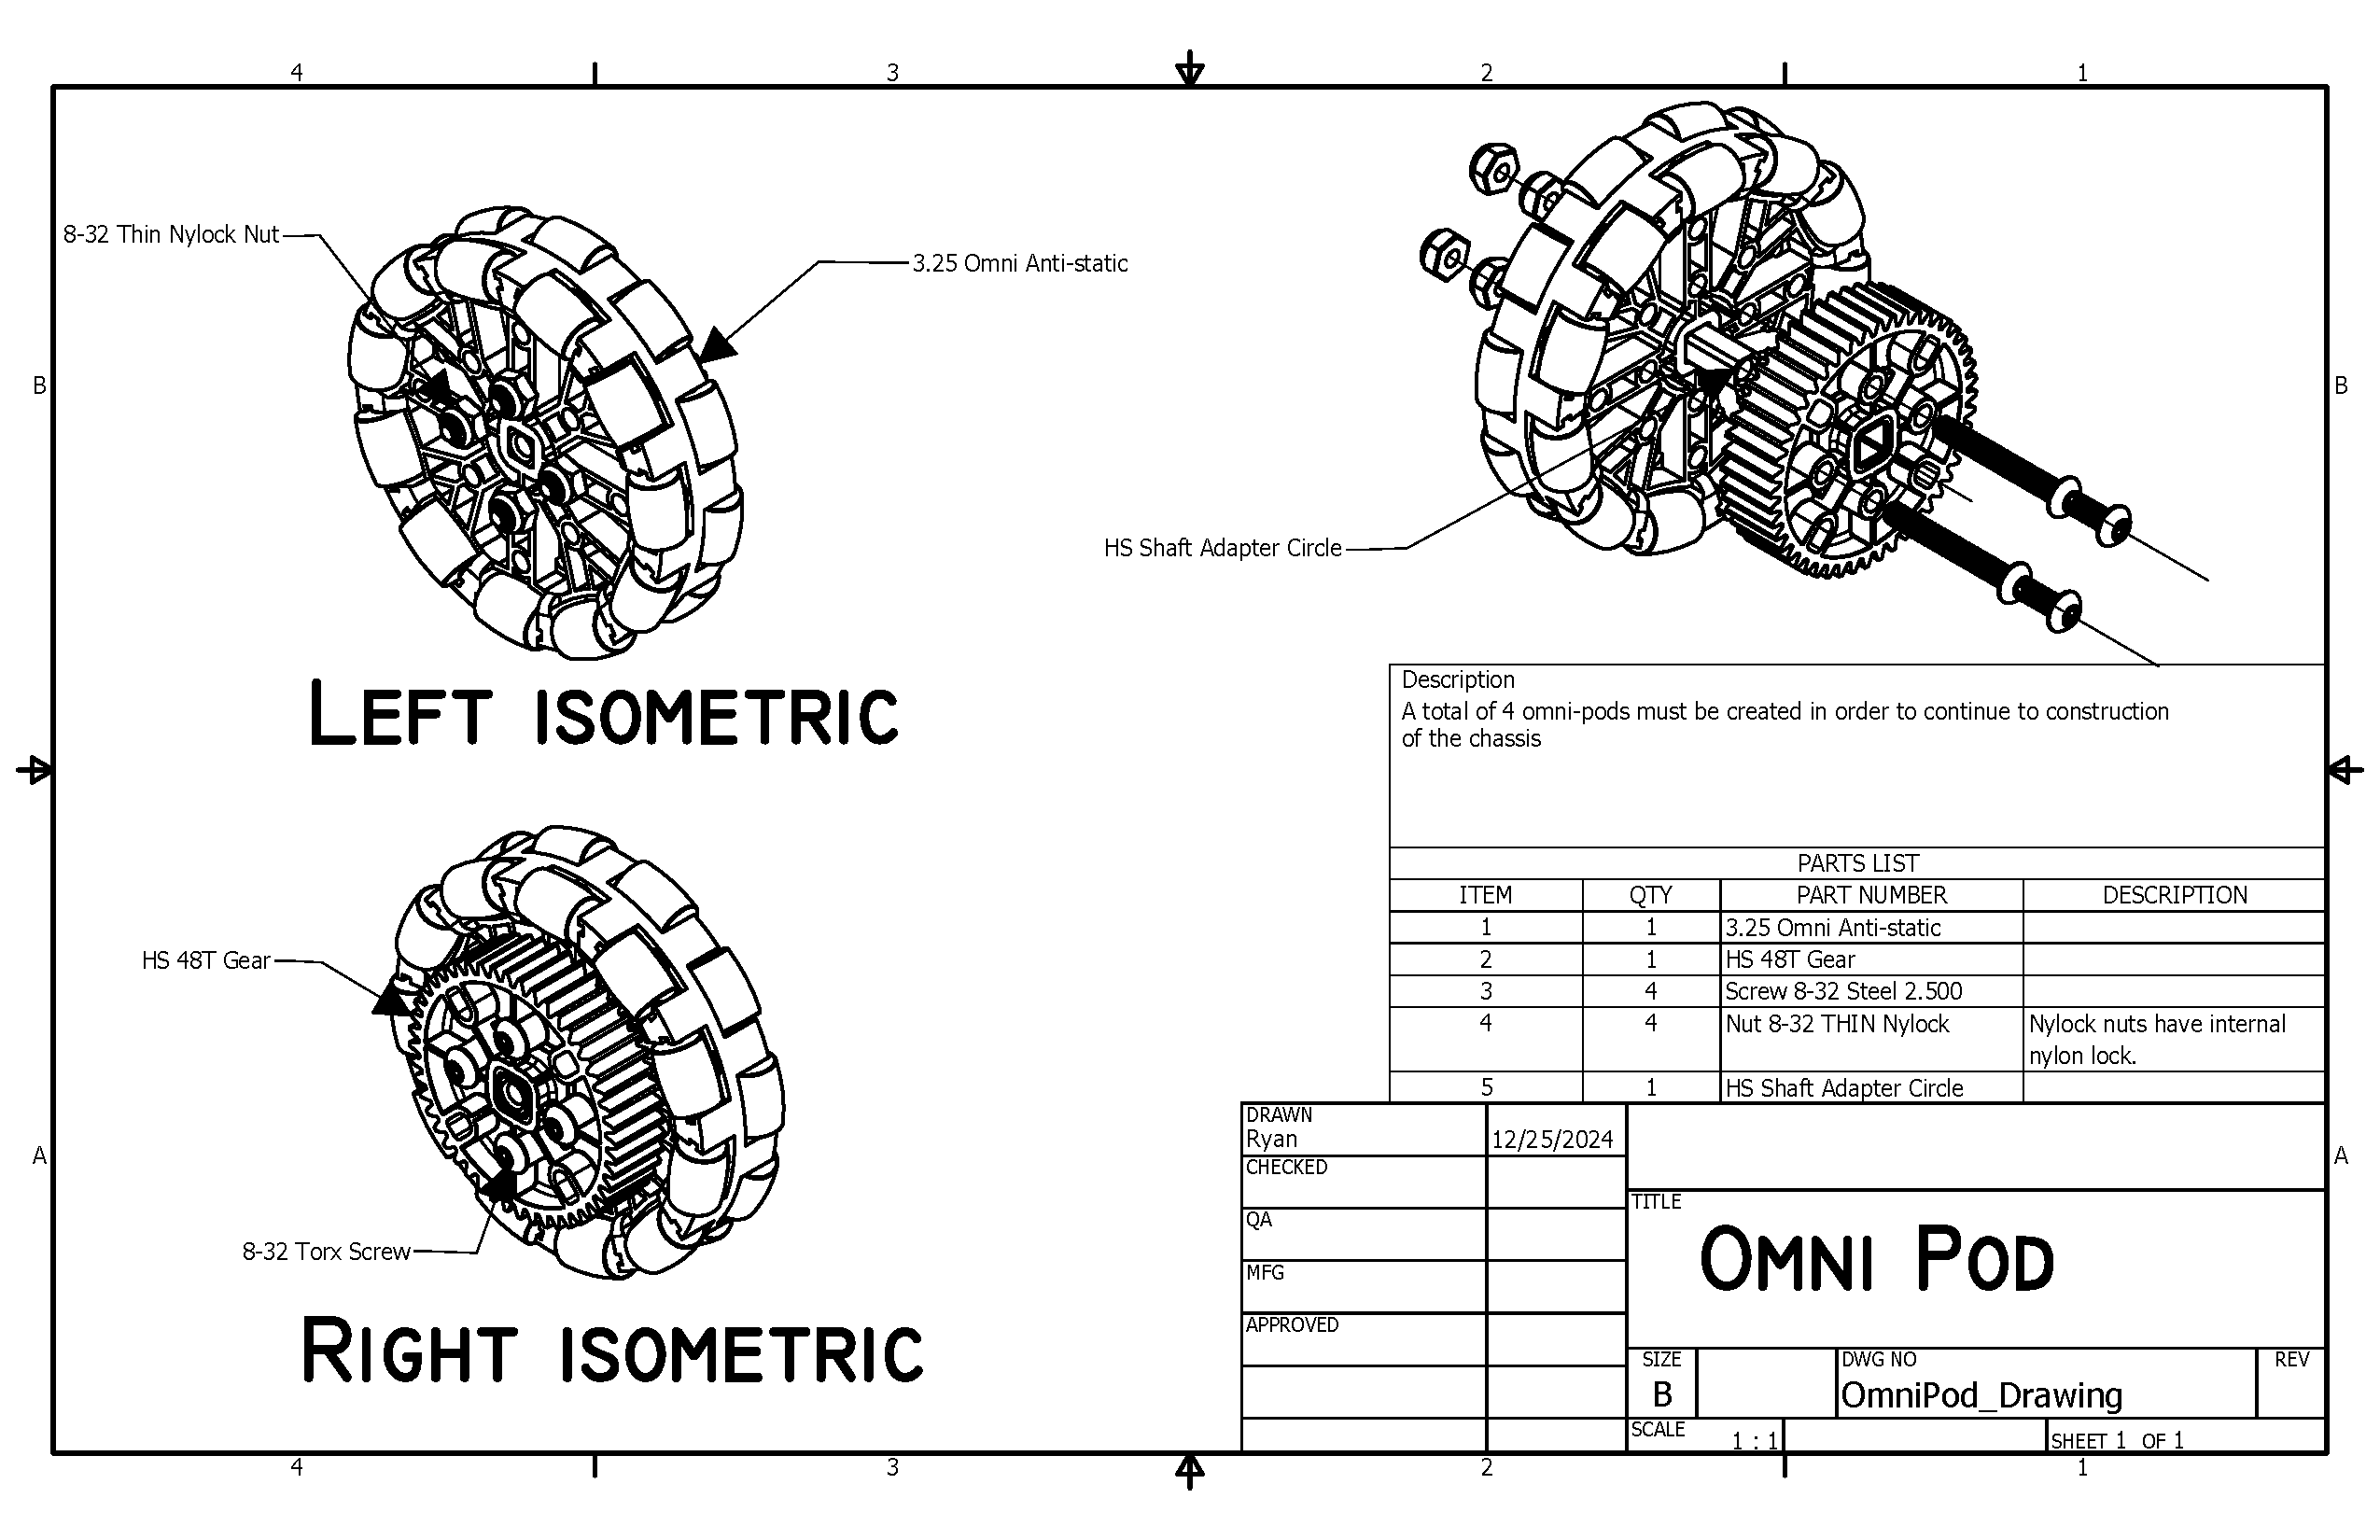
\includegraphics[width=\textheight, angle =90]{images/Subassemblies Drawings and Parts/OmniPod_Drawing.pdf}
    \caption{Enter Caption}
    \label{fig:enter-label}
\end{figure}


\begin{figure}
    \centering
    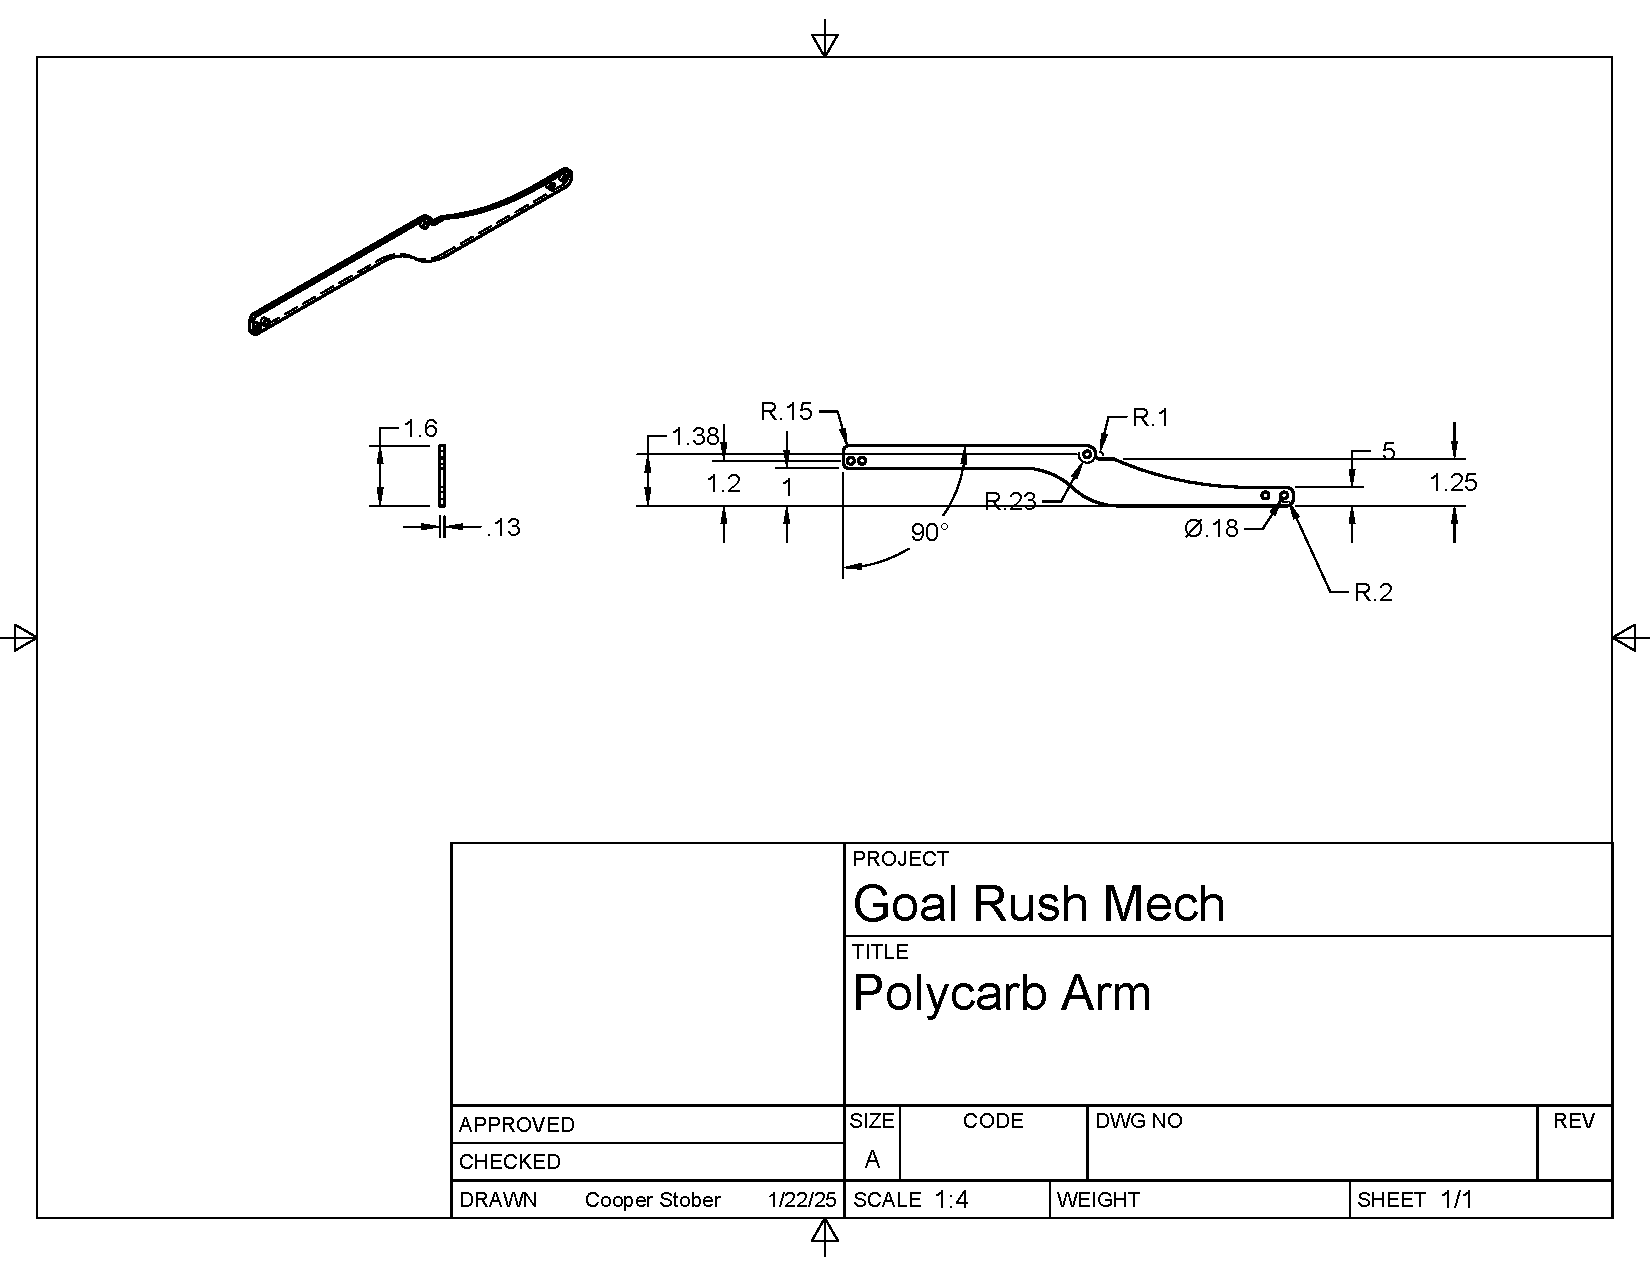
\includegraphics[width=\textheight, angle=90]{images/Subassemblies Drawings and Parts/PolyCarb Drawing.pdf}
    \caption{Enter Caption}
    \label{fig:enter-label}
\end{figure}

\begin{figure}
    \centering
    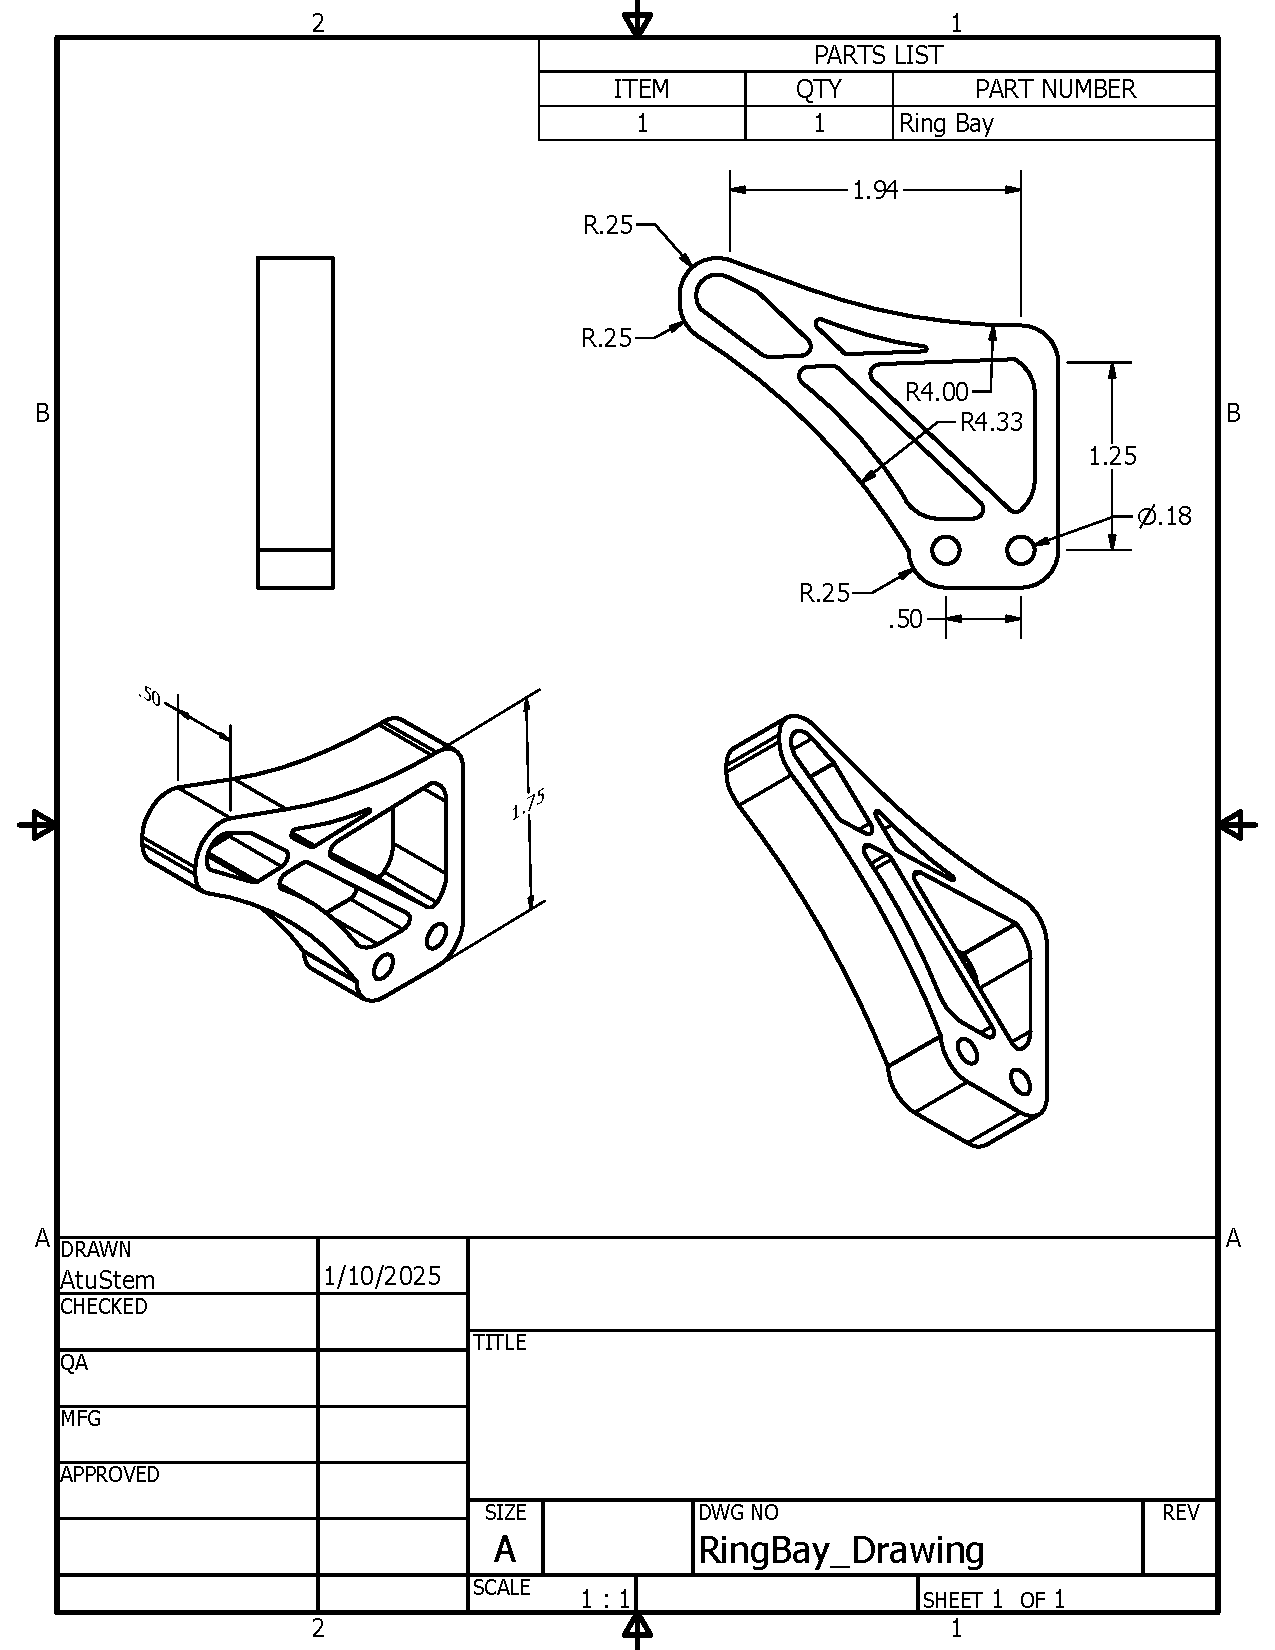
\includegraphics[width=1\linewidth]{images/Subassemblies Drawings and Parts/RingBay_Drawing.pdf}
    \caption{Enter Caption}
    \label{fig:enter-label}
\end{figure}

\begin{figure}
    \centering
    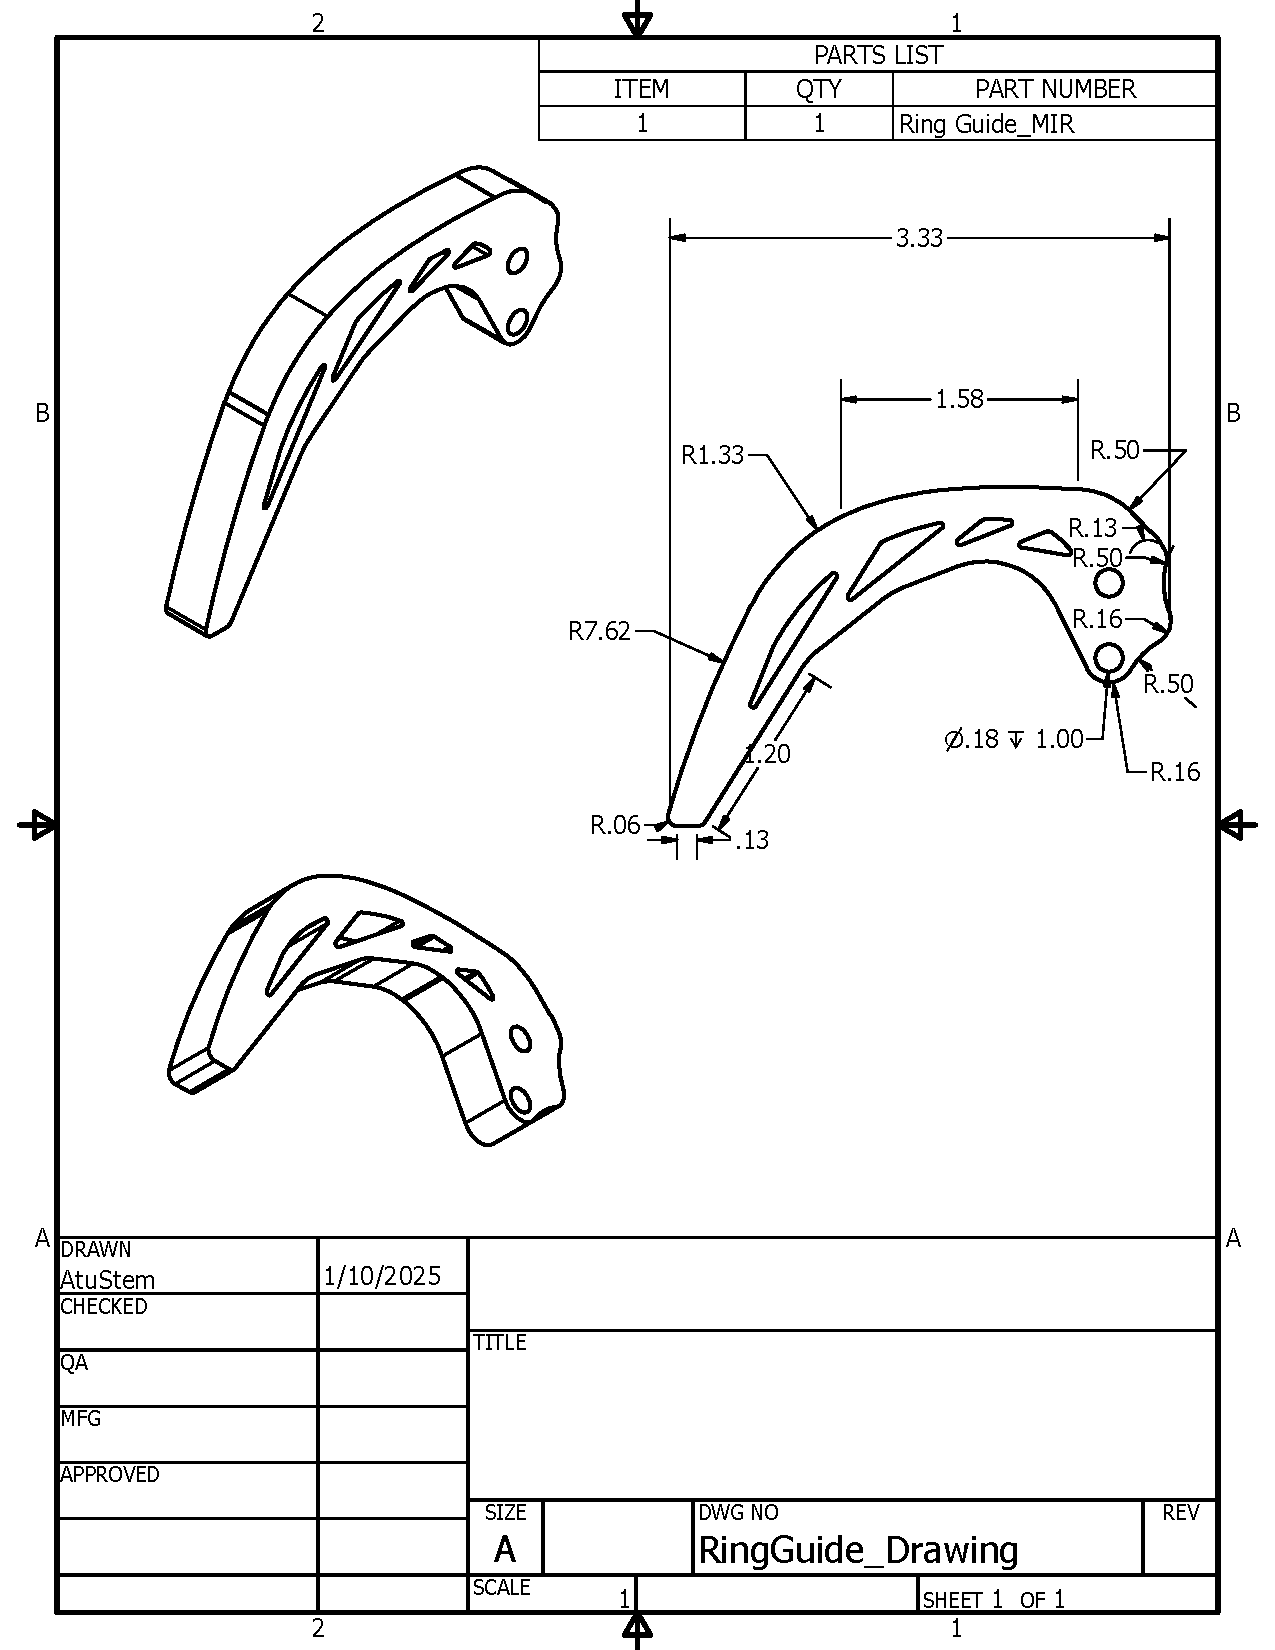
\includegraphics[width=1\linewidth]{images/Subassemblies Drawings and Parts/RingGuide_Drawing.pdf}
    \caption{Enter Caption}
    \label{fig:enter-label}
\end{figure}


\begin{figure}
    \centering
    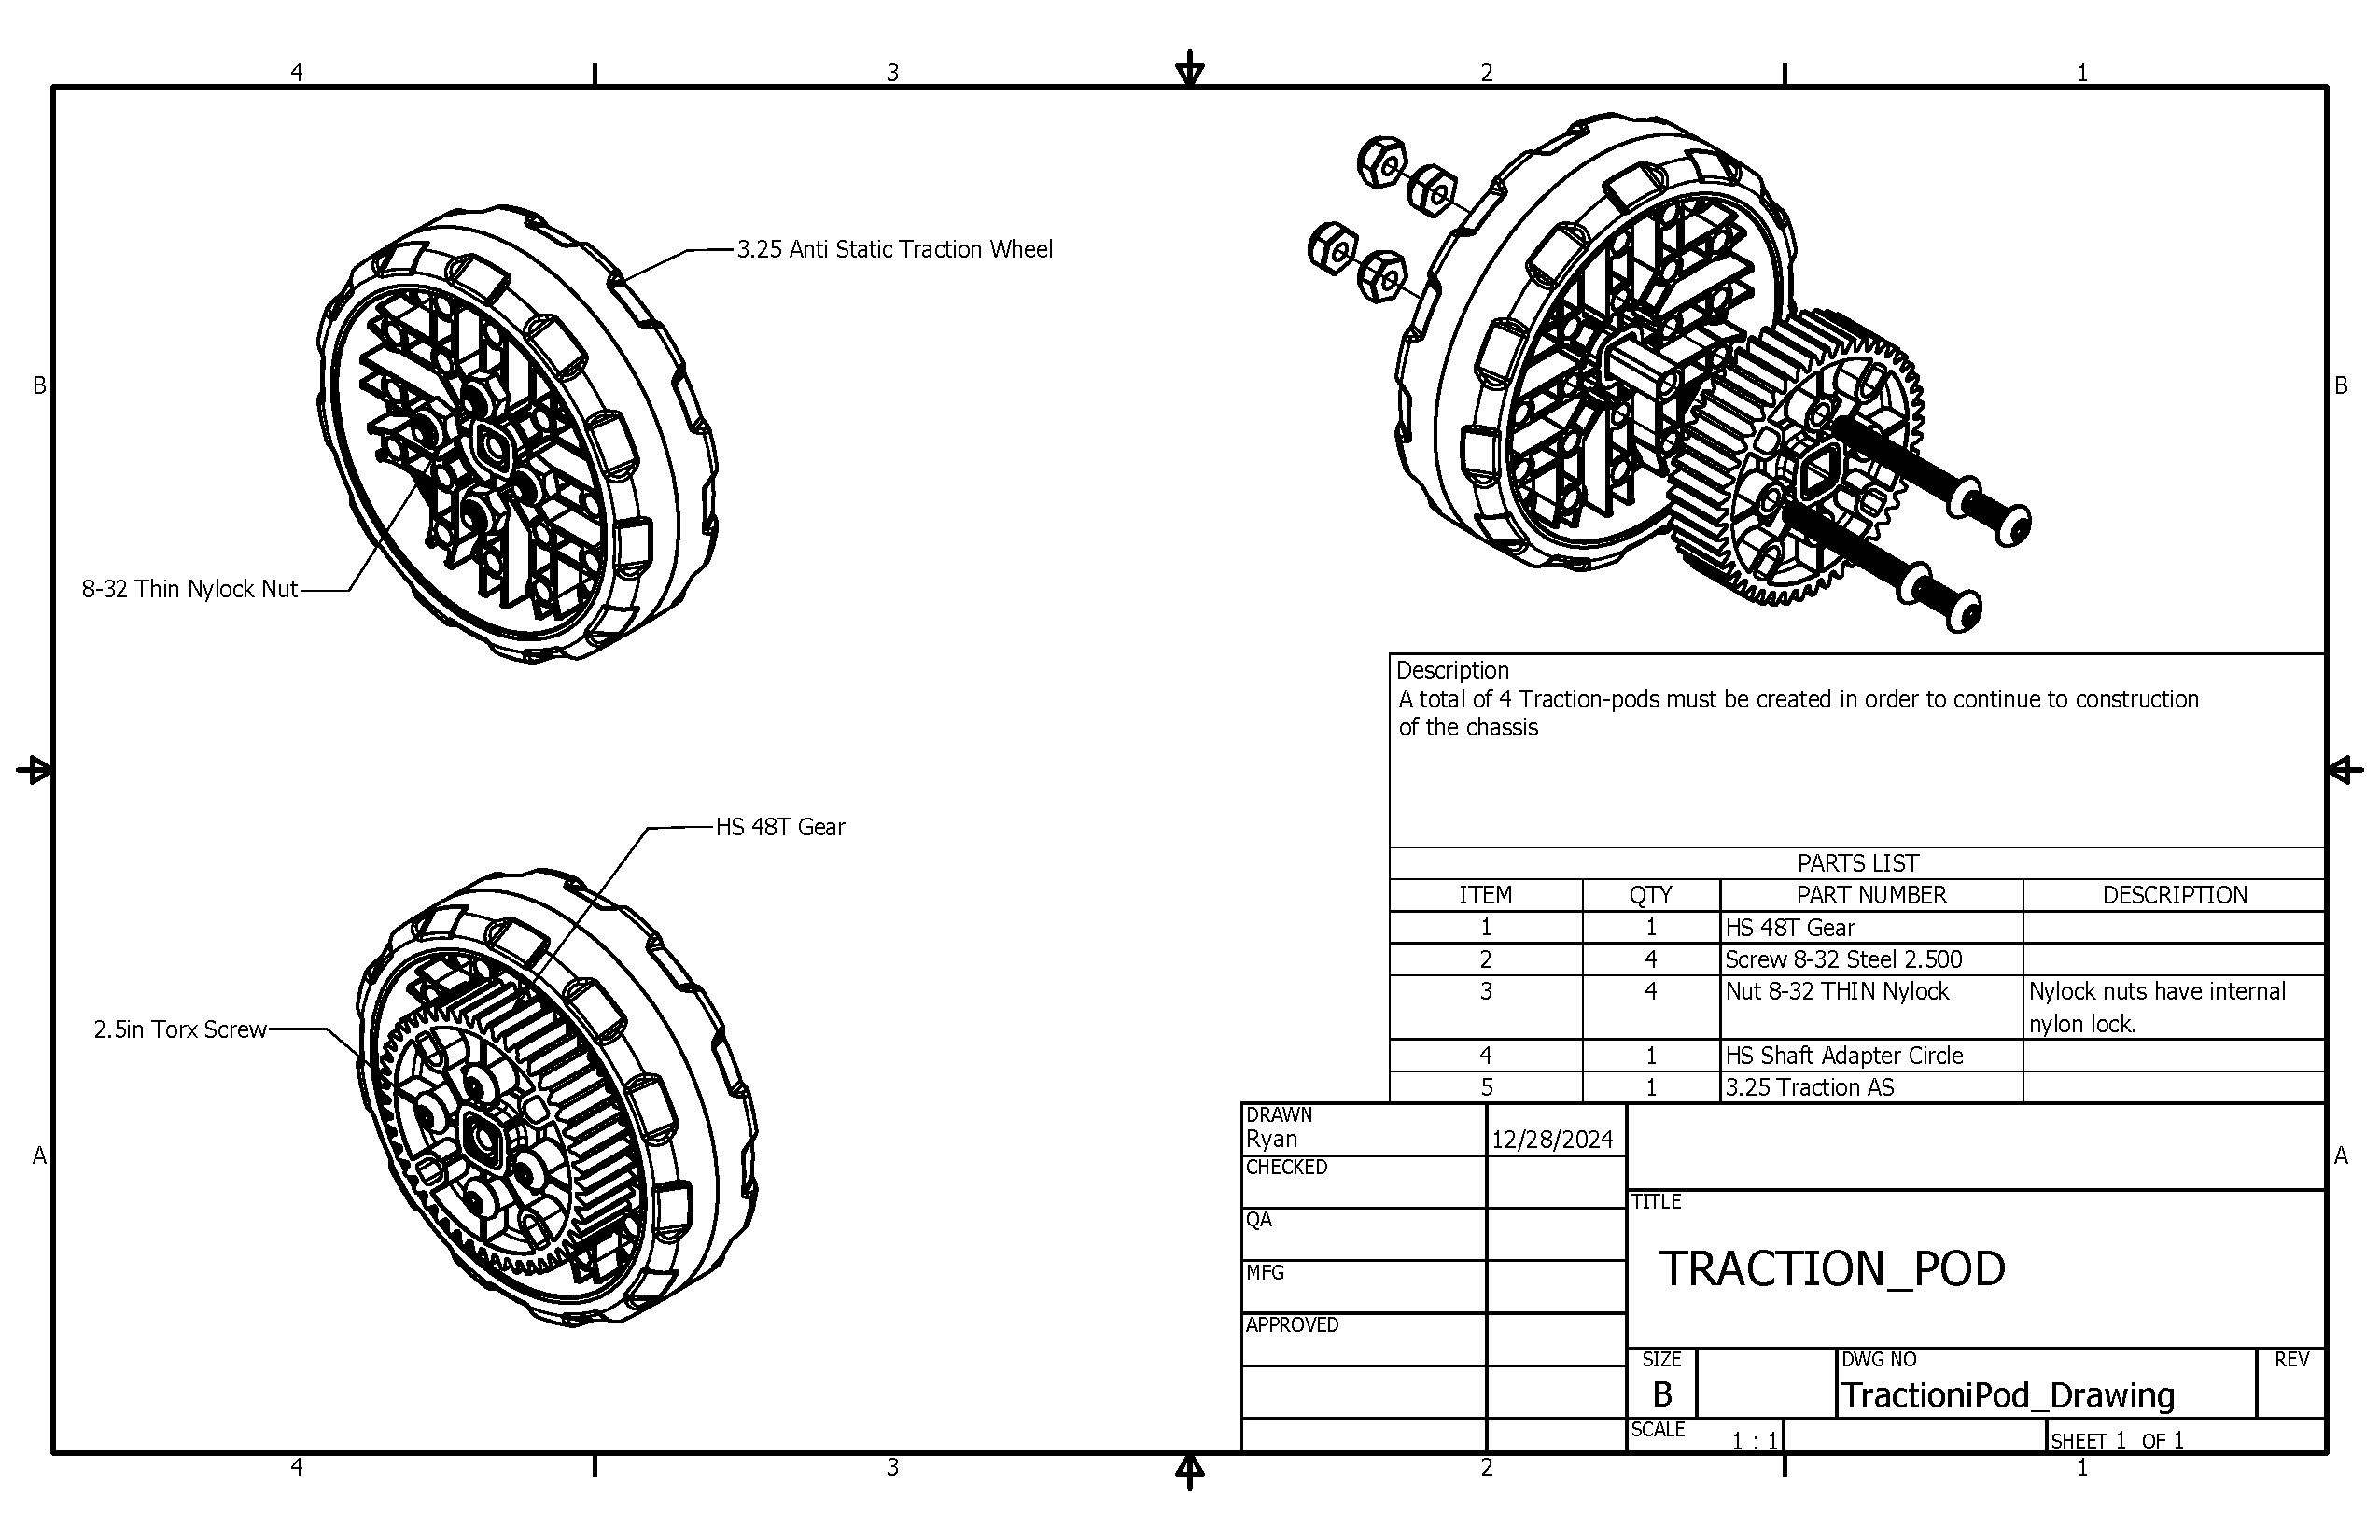
\includegraphics[width=\textheight, angle = 90]{images/Subassemblies Drawings and Parts/TractioniPod_Drawing.pdf}
    \caption{Enter Caption}
    \label{fig:enter-label}
\end{figure}

\addtocontents{toc}{\setcounter{tocdepth}{\defaulttocdepth}}
\setcounter{tocdepth}{\defaulttocdepth}